%==============================================================================
% Tento soubor použijte jako základ
% This file should be used as a base for the thesis
% Autoři / Authors: 2008 Michal Bidlo, 2022 Jaroslav Dytrych
% Kontakt pro dotazy a připomínky: sablona@fit.vutbr.cz
% Contact for questions and comments: sablona@fit.vutbr.cz
%==============================================================================
% kódování: UTF-8 (zmena prikazem iconv, recode nebo cstocs)
% encoding: UTF-8 (you can change it by command iconv, recode or cstocs)
%------------------------------------------------------------------------------
% zpracování / processing: make, make pdf, make clean
%==============================================================================
% Soubory, které je nutné upravit nebo smazat: / Files which have to be edited or deleted:
%   projekt-20-literatura-bibliography.bib - literatura / bibliography
%   projekt-01-kapitoly-chapters.tex - obsah práce / the thesis content
%   projekt-01-kapitoly-chapters-en.tex - obsah práce v angličtině / the thesis content in English
%   projekt-30-prilohy-appendices.tex - přílohy / appendices
%   projekt-30-prilohy-appendices-en.tex - přílohy v angličtině / appendices in English
%==============================================================================
%\documentclass[]{fitthesis} % bez zadání - pro začátek práce, aby nebyl problém s překladem
%\documentclass[english]{fitthesis} % without assignment - for the work start to avoid compilation problem
%\documentclass[zadani]{fitthesis} % odevzdani do IS VUT a/nebo tisk s barevnými odkazy - odkazy jsou barevné
%\documentclass[english,zadani]{fitthesis} % for submission to the IS VUT and/or print with color links - links are color
%\documentclass[zadani,print]{fitthesis} % pro černobílý tisk - odkazy jsou černé
%\documentclass[english,zadani,print]{fitthesis} % for the black and white print - links are black
\documentclass[zadani,cprint,english]{fitthesis} % pro barevný tisk - odkazy jsou černé, znak VUT barevný
%\documentclass[english,zadani,cprint]{fitthesis} % for the print - links are black, logo is color
% * Je-li práce psaná v anglickém jazyce, je zapotřebí u třídy použít 
%   parametr english následovně:
%   If thesis is written in English, it is necessary to use 
%   parameter english as follows:
%      \documentclass[english]{fitthesis}
% * Je-li práce psaná ve slovenském jazyce, je zapotřebí u třídy použít 
%   parametr slovak následovně:
%   If the work is written in the Slovak language, it is necessary 
%   to use parameter slovak as follows:
%      \documentclass[slovak]{fitthesis}
% * Je-li práce psaná v anglickém jazyce se slovenským abstraktem apod., 
%   je zapotřebí u třídy použít parametry english a enslovak následovně:
%   If the work is written in English with the Slovak abstract, etc., 
%   it is necessary to use parameters english and enslovak as follows:
%      \documentclass[english,enslovak]{fitthesis}

% Základní balíčky jsou dole v souboru šablony fitthesis.cls
% Basic packages are at the bottom of template file fitthesis.cls
% zde můžeme vložit vlastní balíčky / you can place own packages here


% Pro seznam zkratek lze využít balíček Glossaries - nutno odkomentovat i níže a při kompilaci z konzoly i v Makefile (plnou verzi pro Perl, nebo lite)
% The Glossaries package can be used for the list of abbreviations - it is necessary to uncomment also below. When compiling from the console also in the Makefile (full version for Perl or lite)
%\usepackage{glossaries}
%\usepackage{glossary-superragged}
%\makeglossaries 

% Nastavení cesty k obrázkům
% Setting of a path to the pictures
%\graphicspath{{obrazky-figures/}{./obrazky-figures/}}
%\graphicspath{{obrazky-figures/}{../obrazky-figures/}}

%---rm---------------
\renewcommand{\rmdefault}{lmr}%zavede Latin Modern Roman jako rm / set Latin Modern Roman as rm
%---sf---------------
\renewcommand{\sfdefault}{qhv}%zavede TeX Gyre Heros jako sf
%---tt------------
\renewcommand{\ttdefault}{lmtt}% zavede Latin Modern tt jako tt

% vypne funkci šablony, která automaticky nahrazuje uvozovky,
% aby nebyly prováděny nevhodné náhrady v popisech API apod.
% disables function of the template which replaces quotation marks
% to avoid unnecessary replacements in the API descriptions etc.
\csdoublequotesoff

\usepackage{url}

% =======================================================================
% balíček "hyperref" vytváří klikací odkazy v pdf, pokud tedy použijeme pdflatex
% problém je, že balíček hyperref musí být uveden jako poslední, takže nemůže
% být v šabloně
% "hyperref" package create clickable links in pdf if you are using pdflatex.
% Problem is that this package have to be introduced as the last one so it 
% can not be placed in the template file.
\ifWis
\ifx\pdfoutput\undefined % nejedeme pod pdflatexem / we are not using pdflatex
\else
  \usepackage{color}
  \usepackage[unicode,colorlinks,hyperindex,plainpages=false,pdftex]{hyperref}
  \definecolor{hrcolor-ref}{RGB}{223,52,30}
  \definecolor{hrcolor-cite}{HTML}{2F8F00}
  \definecolor{hrcolor-urls}{HTML}{092EAB}
  \hypersetup{
	linkcolor=hrcolor-ref,
	citecolor=hrcolor-cite,
	filecolor=magenta,
	urlcolor=hrcolor-urls
  }
  \def\pdfBorderAttrs{/Border [0 0 0] }  % bez okrajů kolem odkazů / without margins around links
  \pdfcompresslevel=9
\fi
\else % pro tisk budou odkazy, na které se dá klikat, černé / for the print clickable links will be black
\ifx\pdfoutput\undefined % nejedeme pod pdflatexem / we are not using pdflatex
\else
  \usepackage{color}
  \usepackage[unicode,colorlinks,hyperindex,plainpages=false,pdftex,urlcolor=black,linkcolor=black,citecolor=black]{hyperref}
  \definecolor{links}{rgb}{0,0,0}
  \definecolor{anchors}{rgb}{0,0,0}
  \def\AnchorColor{anchors}
  \def\LinkColor{links}
  \def\pdfBorderAttrs{/Border [0 0 0] } % bez okrajů kolem odkazů / without margins around links
  \pdfcompresslevel=9
\fi
\fi
% Řešení problému, kdy klikací odkazy na obrázky vedou za obrázek
% This solves the problems with links which leads after the picture
\usepackage[all]{hypcap}

\usepackage[inkscapeformat=png]{svg}
\usepackage{listings}
\usepackage{verbatimbox}
\usepackage{array}
\usepackage{cprotect}
\usepackage{multirow}  % For multi-row spanning cells
\usepackage{multicol}  % For multi-column spanning cells
\usepackage{booktabs}  % For professional looking tables
\usepackage{xcolor}  % Required for custom colors
\usepackage{subcaption}
\usepackage{wrapfig}

\definecolor{darkgreen}{rgb}{0,0.5,0} % RGB color model

% Define custom language for x86 Assembly
\lstdefinelanguage{x86asm}{
  morekeywords={cmpq, jne, mov, test, je, lea, incq, push, callq, incq, retq, add},
  keywordstyle=\color{blue}\bfseries,
  morecomment=[l]{;}, 
  commentstyle=\color{green}\ttfamily,
  morestring=[b]",   
  stringstyle=\color{red}\ttfamily,
  moredelim=*[directive]\#, 
  moredelim=[is][\color{red}\ttfamily]{<}{>}, 
  alsoletter={\%}, 
  morekeywords=[2]{\%rax,\%rdi,\%rcx,\%rdx, \%rbp, \%r15, \%r14, \%rbx, \%rsi, \%edi, \%rip},  % Register names
  keywordstyle=[2]\color{magenta}, 
}


\lstset{
  language=c,
  basicstyle=\ttfamily\small,
  keywordstyle=\color{blue},
  stringstyle=\color{red},
  commentstyle=\color{darkgreen},
  morecomment=[l][\color{magenta}]{\#}
}


% Define a new language for LLVM, based on the listings package
\lstdefinelanguage{LLVM}{
  keywords={define, void, i32, global, constant, private, unnamed_addr, align, ret, br, label, add, fadd, sub, fsub, mul, fmul, sdiv, udiv, fdiv, phi, store, ptr, alloca, nsw},
  keywordstyle=\color{blue}\bfseries,
  identifierstyle=\color{black},
  sensitive=false, 
  comment=[l]{;}, 
  commentstyle=\color{darkgreen}\ttfamily,
  stringstyle=\color{red}\ttfamily,
  morestring=[b]", 
  morestring=[b]'
}

% Set up the style for LLVM code listings
\lstset{
  inputencoding=utf8,
  extendedchars=true,
  language=LLVM,
  basicstyle=\ttfamily\small,
  backgroundcolor=\color{gray!10},
  frame=single,
  captionpos=b,   
  breaklines=true,   
  breakatwhitespace=false,
}



% Informace o práci/projektu / Information about the thesis
%---------------------------------------------------------------------------
\projectinfo{
  %Prace / Thesis
  project={BP},            %typ práce BP/SP/DP/DR  / thesis type (SP = term project)
  year={2024},             % rok odevzdání / year of submission
  date=\today,             % datum odevzdání / submission date
  %Nazev prace / thesis title
  title.cs={Efektivní instrumentace programů v LLVM},  % název práce v češtině či slovenštině (dle zadání) / thesis title in czech language (according to assignment)
  title.en={Efficient Instrumentation of Programs\\using LLVM Framework}, % název práce v angličtině / thesis title in english
  %title.length={14.5cm}, % nastavení délky bloku s titulkem pro úpravu zalomení řádku (lze definovat zde nebo níže) / setting the length of a block with a thesis title for adjusting a line break (can be defined here or below)
  %sectitle.length={14.5cm}, % nastavení délky bloku s druhým titulkem pro úpravu zalomení řádku (lze definovat zde nebo níže) / setting the length of a block with a second thesis title for adjusting a line break (can be defined here or below)
  %dectitle.length={14.5cm}, % nastavení délky bloku s titulkem nad prohlášením pro úpravu zalomení řádku (lze definovat zde nebo níže) / setting the length of a block with a thesis title above declaration for adjusting a line break (can be defined here or below)
  %Autor / Author
  author.name={Vladimír},   % jméno autora / author name
  author.surname={Hucovič},   % příjmení autora / author surname 
  %author.title.p={Bc.}, % titul před jménem (nepovinné) / title before the name (optional)
  %author.title.a={Ph.D.}, % titul za jménem (nepovinné) / title after the name (optional)
  %Ustav / Department
  department={UITS}, % doplňte příslušnou zkratku dle ústavu na zadání: UPSY/UIFS/UITS/UPGM / fill in appropriate abbreviation of the department according to assignment: UPSY/UIFS/UITS/UPGM
  % Školitel / supervisor
  supervisor.name={Jiří},   % jméno školitele / supervisor name 
  supervisor.surname={Pavela},   % příjmení školitele / supervisor surname
  supervisor.title.p={Ing.},   %titul před jménem (nepovinné) / title before the name (optional)
  supervisor.title.a={},   %titul za jménem (nepovinné) / title after the name (optional)
  % Klíčová slova / keywords
  keywords.cs={výkonnostní analýza, instrumentace při překladu, statická instrumentace, LLVM, Perun, LLVM průchod, LLVM pass plugin}, % klíčová slova v českém či slovenském jazyce / keywords in czech or slovak language
  keywords.en={performance analysis, compile-time instrumentation, static instrumentation, LLVM, Perun, LLVM pass framework, LLVM pass plugin }, % klíčová slova v anglickém jazyce / keywords in english
  %keywords.en={Here, individual keywords separated by commas will be written in English.},
  % Abstrakt / Abstract
  abstract.cs={Cílem této práce je vyvinout nový, efektivní profilovací nástroj, který rozšiřuje sadu nástrojů Perun, která je zaměřena na systematické a dlouhodobé monitorování výkonu softwarových projektů. Nový nástroj je založený na technice instrumentace při překladu, s využitím API systému Pass Framework, který je součástí projektu LLVM. Implementovaný profilovací nástroj sbírá počet vykonání základních bloků v programu. Několik optimalizačních technik, jako je inlining instrumentačního kódu nebo analýza grafu toku řízení funkcí, bylo využito pro snížení profilovací režie tohoto nástroje. Výkon nástroje byl vyhodnocen na dvou projektech a experimenty ukázaly, že jeho profilovací režie je nižší než režie některých existujících open-source nástrojů.}, % abstrakt v českém či slovenském jazyce / abstract in czech or slovak language
  abstract.en={The goal of this thesis is to develop a new, efficient profiler to extend the Perun tool suite, which focuses on systematic and long-term performance monitoring of software projects. The new profiler is based on a technique of compile-time instrumentation using the Pass Framework API within the LLVM compiler infrastructure project. The implemented profiler focuses on collecting the number of executions of each basic block in the program. Several optimization techniques, including inlining instrumentation code and function control flow graph analysis were used to reduce the runtime overhead of the profiler. The performance of the profiler was evaluated on two real-world projects and experiments have shown that it achieved lower profiling overhead than some established open-source tools.}, % abstrakt v anglickém jazyce / abstract in english
  %abstract.en={An abstract of the work in English will be written in this paragraph.},
  % Prohlášení (u anglicky psané práce anglicky, u slovensky psané práce slovensky; u projektové praxe lze zakomentovat) / Declaration (for thesis in english should be in english; for project practice can be commented out)
  declaration={I hereby declare that this bachelor’s thesis was prepared as an original work by the author
under the supervision of Ing. Jiří Pavela and Ing. Tomáš Fiedor, Ph.D. I have listed all the literary sources,
publications and other sources, which were used during the preparation of this thesis.
 },
  %declaration={I hereby declare that this Bachelor's thesis was prepared as an original work by the author under the supervision of Mr. X
% The supplementary information was provided by Mr. Y
% I have listed all the literary sources, publications and other sources, which were used during the preparation of this thesis.},
  % Poděkování (nepovinné, nejlépe v jazyce práce; nechcete-li, zakomentujte pro skrytí nadpisu) / Acknowledgement (optional, ideally in the language of the thesis; comment out for hiding including heading)
  acknowledgment={I would like to thank Ing. Jiří Pavela and Ing. Tomáš Fiedor, Ph.D. for providing me with excellent guidance, advice, and feedback. I would also like to thank my friends and family for always supporting me in pursuing my academic goals. },
  %acknowledgment={Here it is possible to express thanks to the supervisor and to the people which provided professional help
%(external submitter, consultant, etc.).},
  % Rozšířený abstrakt (cca 3 normostrany) - lze definovat zde nebo níže / Extended abstract (approximately 3 standard pages) - can be defined here or below
  extendedabstract={
Výkon spotřebitelských aplikací je významným faktorem uživatelské zkušenosti, jak ukazují studie zaměřené na analýzu výkonu webových stránek a spokojenosti zákazníků, přičemž 79\% uživatelů, kteří byli nespokojeni s výkonem webové stránky při jejich první návštěvě, ji pravděpodobně nikdy znovu nenavštíví. Stačí jednosekundové zpoždění načítání stránky internetového obchodu, aby míra konverze zákazníků klesla o 7\% \cite{performance-ux}.

Provozování efektivnějších aplikací v datových centrech by mohlo pomoci snížit jejich spotřebu energie, která by podle některých předpovědí měla do roku 2030 dosáhnout 3 biliony kWh ročně, oproti méně než 500 miliardám kWh v roce 2010 \cite{datacenter-energy}.

Výkon softwaru je také důležitý ve vestavěných a mobilních systémech, kde jsou zdroje omezené a zařízení jsou běžně poháněna bateriemi s omezenou kapacitou. Optimalizováním aplikací mohou vývojáři zlepšit výdrž baterie na jedno nabití a s tím i životnost baterie.~\cite{embedded}

Po desetiletí byla neustále rostoucí poptávka po výpočetním výkonu kompenzována \emph{Mooreovým zákonem}, předpovědí spoluzakladatele společnosti Intel Gordona Moorea, že počet tranzistorů na čipech se bude každé dva roky zdvojnásobovat. V poslední době se objevily známky, že Mooreův zákon zpomaluje, protože návrháři čipů se blíží fyzikálním limitům. Nelze ale říci, že by požadavky moderních aplikací na stále více výpočetních zdrojů zpomalovaly s ním. \cite{moores-law-1, moores-law-2-woods}.

Aby vývojáři vyhověli požadavkům na výkon aplikací ve světě, který se již neřídí Mooreovým zákonem, budou muset věnovat více času a pozornosti optimalizaci aplikací a předcházení výkonnostní degradaci. Specializované nástroje jsou nezbytné pro sběr, interpretaci a vizualizaci výkonnostních dat,  stejně jako pro monitoring výkonu softwarových projektů během celého vývojového cyklu. Jedním z prostředků vyvinutých pro tento účel je open-source sada nástrojů Perun \cite{perun-paper}.

Většina profilerů používaných v sadě nástrojů Perun je založena na dobře zavedené technice profilování: instrumentaci. I když instrumentace nabízí velkou flexibilitu co se týče rozsahu dostupných metrik, které lze měřit v různé granularitě, dosahuje toho za cenu vysoké režie. Tato režie by mohla být omezena použitím technik, jako je instrumentace při překladu.

V rámci této práce jsme vytvořili nový profilovací nástroj, který rozšíří sadu nástrojů Perun. Tento nový nástroj se zaměřuje na efektivní profilování počtu vykonaných instrukcí v programech napsaných v jazycích C a C++ s granularitou na úrovni základních bloků, přičemž minimalizuje režii využitím optimalizačních technik specifických pro profilování založené na instrumentaci při překladu.

Celkem byly vyvinuty a porovnány 4 verze nástroje. Nejprve byly optimalizovány datové struktury, do kterých se při profilování ukládají informace, aby režie spojená se zápisem do těchto struktur byla co nejnižší. Volání instrumentačních funkcí bylo nahrazeno inline instrumentací. V neposlední řadě bylo využito statické analýzy grafu toku řízení pro snížení počtu instrumentačních bodů, aniž by byla ovlivněna přesnost výsledného profilu. Kromě nástroje samotného byla vyvinuta i interaktivní vizualizace naměřených dat.

Vyvinutý nástroj byl vyhodnocen na dvou open-source projektech, kompresním nástroji \texttt{CCSDS} a interpretu \texttt{CPython}. Experimenty ukázaly, že oproti první verzi nástroje byla režie snížena o více než 90\%. Nástroj byl porovnán se dvěma open-source profilovacími nástroji \texttt{Callgrind} a \texttt{gprof}. Výsledky ukázaly, že optimalizovaná verze nástroje dosahuje nižší režie, než tyto zavedené nástroje.

},
  %extabstract.odd={true}, % Začít rozšířený abstrakt na liché stránce? / Should extended abstract start on the odd page?
  %faculty={FIT}, % FIT/FEKT/FSI/FA/FCH/FP/FAST/FAVU/USI/DEF
  faculty.cs={Fakulta informačních technologií}, % Fakulta v češtině - pro využití této položky výše zvolte fakultu DEF / Faculty in Czech - for use of this entry select DEF above
  faculty.en={Faculty of Information Technology}, % Fakulta v angličtině - pro využití této položky výše zvolte fakultu DEF / Faculty in English - for use of this entry select DEF above
  department.cs={Ústav matematiky}, % Ústav v češtině - pro využití této položky výše zvolte ústav DEF nebo jej zakomentujte / Department in Czech - for use of this entry select DEF above or comment it out
  department.en={Institute of Mathematics} % Ústav v angličtině - pro využití této položky výše zvolte ústav DEF nebo jej zakomentujte / Department in English - for use of this entry select DEF above or comment it out
}

% Rozšířený abstrakt (cca 3 normostrany) - lze definovat zde nebo výše / Extended abstract (approximately 3 standard pages) - can be defined here or above
%\extendedabstract{Do tohoto odstavce bude zapsán výtah (abstrakt) práce v českém (slovenském) jazyce.}
% Začít rozšířený abstrakt na liché stránce? / Should extended abstract start on the odd page?
%\extabstractodd{true}

% nastavení délky bloku s titulkem pro úpravu zalomení řádku - lze definovat zde nebo výše / setting the length of a block with a thesis title for adjusting a line break - can be defined here or above
%\titlelength{14.5cm}
% nastavení délky bloku s druhým titulkem pro úpravu zalomení řádku - lze definovat zde nebo výše / setting the length of a block with a second thesis title for adjusting a line break - can be defined here or above
%\sectitlelength{14.5cm}
% nastavení délky bloku s titulkem nad prohlášením pro úpravu zalomení řádku - lze definovat zde nebo výše / setting the length of a block with a thesis title above declaration for adjusting a line break - can be defined here or above
%\dectitlelength{14.5cm}

% řeší první/poslední řádek odstavce na předchozí/následující stránce
% solves first/last row of the paragraph on the previous/next page
\clubpenalty=10000
\widowpenalty=10000

% checklist
\newlist{checklist}{itemize}{1}
\setlist[checklist]{label=$\square$}

% Kompilace po částech (rychlejší, ale v náhledu nemusí být vše aktuální)
% Compilation piecewise (faster, but not all parts in preview will be up-to-date)
% Další informace viz / For more information see https://www.overleaf.com/learn/latex/Multi-file_LaTeX_projects
% \usepackage{subfiles}

% Nechcete-li, aby se u oboustranného tisku roztahovaly mezery pro zaplnění stránky, odkomentujte následující řádek / If you do not want enlarged spacing for filling of the pages in case of duplex printing, uncomment the following line
% \raggedbottom

\begin{document}
  % Vysazeni titulnich stran / Typesetting of the title pages
  % ----------------------------------------------
  \maketitle
  % Obsah
  % ----------------------------------------------
  \setlength{\parskip}{0pt}

  {\hypersetup{hidelinks}\tableofcontents}
  
  % Seznam obrazku a tabulek (pokud prace obsahuje velke mnozstvi obrazku, tak se to hodi)
  % List of figures and list of tables (if the thesis contains a lot of pictures, it is good)
  \ifczech
    \renewcommand\listfigurename{Seznam obrázků}
  \fi
  \ifslovak
    \renewcommand\listfigurename{Zoznam obrázkov}
  \fi
  %{\hypersetup{hidelinks}\listoffigures}
  
  \ifczech
    \renewcommand\listtablename{Seznam tabulek}
  \fi
  \ifslovak
    \renewcommand\listtablename{Zoznam tabuliek}
  \fi
  % {\hypersetup{hidelinks}\listoftables}

  % Seznam zkratek / List of abbreviations
  %\ifczech
  %  \renewcommand*\glossaryname{Seznam zkratek}%
  %  \renewcommand*\entryname{Zkratka}
  %  \renewcommand*\descriptionname{Význam}
  %\fi
  %\ifslovak
  %  \renewcommand*\glossaryname{Zoznam skratiek}%
  %  \renewcommand*\entryname{Skratka}
  %  \renewcommand*\descriptionname{Význam}
  %\fi
  %\ifenglish
  %  \renewcommand*\glossaryname{List of abbreviations}%
  %  \renewcommand*\entryname{Abbreviation}
  %  \renewcommand*\descriptionname{Meaning}
  %\fi
  % Definice zkratek - z textu se odkazují např. \Gls{TF–IDF}
  % Definition of abbreviations - referred from the text e.g. \Gls{TF–IDF}
  %\newglossaryentry{TF–IDF}
  %{
  %  name={TF–IDF},
  %  description={Term Frequency-Inverse Document Frequency}
  %}
  % 
  %\setglossarystyle{superragged}
  %\printglossaries


  \ifODSAZ
    \setlength{\parskip}{0.5\bigskipamount}
  \else
    \setlength{\parskip}{0pt}
  \fi

  % vynechani stranky v oboustrannem rezimu
  % Skip the page in the two-sided mode
  \iftwoside
    \cleardoublepage
  \fi

  % Text prace / Thesis text
  % ----------------------------------------------
  \ifenglish
    % This file should be replaced with your file with an thesis content.
%=========================================================================
% Authors: Michal Bidlo, Bohuslav Křena, Jaroslav Dytrych, Petr Veigend and Adam Herout 2019

% For compilation piecewise (see projekt.tex), it is necessary to uncomment it and change
% \documentclass[../projekt.tex]{subfiles}
% \begin{document}

\chapter{Introduction}
\label{intro}

%In 1965, the co-founder and former CEO of Intel, Gordon Moore, noticed a trend of the number of transistors on chips doubling every year. He predicted that this trend would continue far into the future, later revising his prediction in 1975 to transistor count doubling every two years. This prediction, known as \emph{"Moore's law,"} has held strong for several decades, driving exponential growth in computer performance from the tireless efforts of semiconductor researchers and engineers. At the same time, however, the appetite of modern applications for ever more computing resources has kept up with Moore's law, driven not just by legitimate demand coming from High-Performance Computing (HPC) applications such as scientific calculations or weather prediction models \cite{weather-prediction-models}, but also by increasingly bloated and inefficient applications, development processes that prioritize other concerns before performance, and higher-level programming languages which substantially increase the execution time of algorithms compared to their low-level counterparts, with a simple matrix multiplication program running 47 times longer when written in Python compared to the same program written in C. \cite{moores-law-1}

%In recent years, as the limits of physics are being approached and the size of transistors inches closer to atomic levels, Moore's law appears to be slowing down. It took Intel 5 years to go from 14nm manufacturing technology, developed in 2014, to 10nm in 2019, rather than the two years it should take according to Moore's prediction \cite{moores-law-2-woods}. There is, however, no evidence that the demand for ever more computing power is slowing down with it.

The performance of consumer applications is a significant factor in user experience, as shown by studies focused on analyzing website performance and customer satisfaction, with 79\% of users who were dissatisfied with website performance on their first visit being less likely ever to use it again. Additionally, it takes just a one-second delay in page loading time on an e-commerce website for the customer conversion rate to drop by 7\% 
\cite{performance-ux}.

Running more efficient applications in data center and cloud computing environments could help reduce their energy consumption, which is, according to some predictions, on track to reach 3 trillion kWh per year by  2030, up from less than 500 billion in 2010 \cite{datacenter-energy}. 

Better software performance is also important in embedded and mobile systems, where resources are scarce, and devices are commonly powered by batteries with limited capacities. By optimizing applications to be more efficient, developers can improve the battery life of these devices and the lifespan of the batteries \cite{embedded}.

For decades, the ever-increasing demand for computing power has been compensated by \emph{Moore's law}, a prediction made by the co-founder of Intel, Gordon Moore, that the number of transistors on chips would double every two years. Recently, there have been signs that Moore's law might be slowing down as chip designers are approaching the limits of physics. There is, however, no evidence that the appetite of modern applications for more computing power is slowing down with it. \cite{moores-law-1, moores-law-2-woods}.

To meet demands on application performance, developers in post-Moore's law world will have to dedicate more time and attention to optimizing applications and avoiding performance degradation. Specialized tools are necessary for the purpose of collecting, interpreting, and visualizing performance-related data, as well as performance monitoring of software projects throughout their development life cycle. One of the tools developed for this purpose is the open-source tool suite Perun \cite{perun-paper}, built specifically with continuous integration and long-term performance monitoring in mind.

Most of the profilers used in Perun's tool suite are based on a well-established profiling technique: instrumentation. While instrumentation offers great flexibility in terms of the range of available metrics that can be measured at various granularities, it comes at a price of substantial overhead. This overhead could be limited by using more lightweight techniques, such as compile-time instrumentation.

This work aims to create a new profiling tool to extend Perun's tool suite. This new tool focuses on efficiently profiling the number of executed instructions in C/C++ programs with basic-block-level granularity while minimizing overhead by taking advantage of optimization techniques specific to profiling based on compile-time instrumentation. 


\medskip
\noindent

\textbf{Sturcture of the thesis}. Chapter \ref{performance-analysis} introduces common profiling techniques, their unique advantages and tradeoffs. Chapter \ref{perun} describes the Perun tool suite, its architecture, and the currently implemented performance data collectors. Chapter \ref{llvm} provides an overview of the architecture of the LLVM Compiler Infrastructure, which is used by the implemented profiler for instrumentation through its Pass Framework. Chapter \ref{implementation} describes the design and implementation of the profiler, with a focus on the techniques used to improve its performance by reducing runtime overhead. This chapter also contains an experimental evaluation of the profiler on two projects, highlighting the incremental improvements in usability and runtime overhead in each version. Chapter \ref{visualizations} shows the implemented visualizations of collected data. Chapter \ref{compare} compares the performance of the implemented profiler with two established open-source profilers. Chapter \ref{conclusion} summarises the results and discusses potential future work.


\chapter{Performance Analysis}
\label{performance-analysis}

In a book written by an acclaimed performance expert, Brendan Gregg, \emph{Systems Performance and the Cloud} \cite{gregg-systems-performance}, Gregg describes \emph{profiling} as `\emph{use of tools that perform sampling: taking a subset of measurements to paint a coarse picture of the target}.' In this thesis, the word `profiling' will be used to describe the overarching process of dynamic performance analysis and testing, similar to publications like \cite{nethercote-dyn-bin}. In this context, profiling is a technique that software engineers use to analyze the behavior of a program by collecting various performance-related metrics, such as time, memory or power consumption, I/O utilization, and others.

Performance analysis has become crucial in modern software development. Computers nowadays are much more complex than just a few decades ago, and it is near impossible for programmers to accurately assess how exactly their program interacts with the hardware executing it. Specialized tools, called profilers, aim to solve this problem. Profilers collect the required performance data about the program, which engineers can then interpret and utilize to tweak the program to improve its performance.

This chapter first introduces instrumentation as an essential technique used in many modern profilers. We compare different approaches to instrumentation and describe their advantages and disadvantages. Finally, we provide an overview of other common profiling techniques, summarize their characteristics, and provide example tools that utilize each technique. 


\section{Instrumentation}

Instrumentation involves modifying an existing program by adding additional code (further referred to as `instrumentation code'). This can be done manually by the programmer or by an automated tool that operates with a predefined instrumentation policy. For example, the policy might dictate that a call to an instrumentation function is inserted before and after each function call.

The advantage of using instrumentation-based techniques for profiling is the level of detail that the analysis can provide. By using custom instrumentation functions, all kinds of information about the running program can be recorded at various points of its execution, with various levels of granularity\footnote{Granularity refers to the level of detail that the method provides, e.g., a profiling method with function-level granularity can provide performance information about functions, but cannot distinguish finer details within those functions, such as lines of code or individual instructions.}. However, the main drawback is the overhead introduced by the additional code, which can significantly affect the program's performance and may not be suitable for profiling in production environments. Since instrumentation modifies the program, it may introduce side effects, such as cache pollution, which could cause useful program data to be evicted from the cache in favor of data related to the instrumentation code. As a result, it may produce distortions in the collected performance data.

\subsection{Static instrumentation}
Static instrumentation involves inserting code into a program before it runs or compiles. This type of instrumentation can take place at the source-code level, as is typically the case with manually added instrumentation points or with tools that specialize in the automatic instrumentation of code written in a particular language. The advantage of this approach is that the tool has complete access to all source-level information. This can be used for detailed analysis before any instrumentation is performed, possibly leading to more efficient instrumentation. The obvious disadvantage is the lack of flexibility \,--\, it can only be used for one source language. The added instrumentation code also increases the size of the resulting executable file.

More commonly, static instrumentation takes place at the binary level. That involves disassembling the executable file or object files, inserting instrumentation code, and reassembling the binary again. This approach is used, e.g., by the \texttt{PEBIL} tool \cite{pebil}.

A middle ground between these two approaches is the instrumentation of an intermediate representation (IR) language, which compilers use to perform internal analyses and transformations, especially optimizations \cite{advanced-compiler-design}. Intermediate representations retain more information about the original code, which can be used for more detailed analysis before performing the instrumentation. At the same time, however, they can be source-language-agnostic, which lends them more flexibility than the instrumentation of high-level source code.


\subsection{Dynamic instrumentation}
Dynamic instrumentation refers to rewriting the executable code at runtime. Therefore, this instrumentation can only be done at the binary level. This is done either by using a wrapper over the analyzed program, an external process, or tools provided by the operating system, e.g., \emph{uprobes} or \emph{kprobes} in Linux, described in Section \ref{tracing}. The major advantage of this approach is that it is usable for programs that utilize dynamically generated code, and provides full coverage of the target, including dynamically loaded libraries. It also typically does not require any preparation of the profiled program, making it very convenient for users. The disadvantage is that the cost of instrumentation is incurred at runtime. Additionally, when handling the instrumentation routines, the program has to be paused, its state (such as the contents of registers) saved and then restored once the routines have been completed. These factors make it one of the slowest methods of dynamic analysis. \emph{Valgrind}, SystemTap, and \emph{Intel Pin} are examples of popular tools that utilize dynamic instrumentation. \cite{valgrind, nethercote-dyn-bin}

\section{Statistical profiling}

Another notable technique is statistical profiling, sometimes referred to as just \emph{sampling}.
This method does not typically require instrumentation of the program: it merely samples the program's stack trace or the CPU's instruction pointer at set intervals. The major advantage of this technique is that the added overhead is minimal compared to other techniques. Since the code of the program is not modified, this method can avoid some side effects of instrumentation-based methods. The disadvantage is that the resulting profile is not a completely accurate representation of the program's performance, and the degree of inaccuracy depends on the sampling rate. Increasing the sampling rate will improve accuracy but incurs additional overhead \cite{bpf-tools}. An example of a tool that provides statistical profiling capabilities is the Linux tool \emph{perf}.

\section{Tracing}
\label{tracing}
Tracing is an event-based approach to profiling, where each instance of an event in a set of events is recorded. This recording produces a program's trace \,--\, a complete picture of the events that took place during the program's run. The disadvantage of tracing is that it can be very expensive in terms of overhead, depending on the rate of the observed events. Tracing also often produces a large amount of data, which takes up a lot of disk space, and the post-processing required to interpret the collected data can be very time-consuming. Linux tools \emph{strace} and \emph{ftrace} are examples of tracing profilers. The former is designed to trace system calls and incoming signals, while the latter traces function calls. 

Some tracing tools utilize kernel \emph{tracepoints}, static probes inserted into logical execution points inside the Linux kernel. They provide a stable interface, which means that robust tools can be built around them. Their advantage is that the overhead is very small, though this largely depends on the rate of events. They can also be disabled, transforming them into no-op instructions, causing only negligible overhead.

Other tools utilize \emph{kprobes}, which are probes based on dynamic instrumentation \,--\, they expose raw kernel functions and arguments that can change between kernel versions. There is also a user-space variant of kprobes, called \emph{uprobes}, which dynamically instrument functions in applications and libraries. \cite{gregg-systems-performance} 

\subsection{Hardware tracing}
Some CPU manufacturers provide hardware CPU tracing on their architectures. This includes tools such as Intel Processor Trace \cite{int-proc-trace} or AMD $\mu{Prof}$ \cite{uprof}. Because of the tight integration with the CPU and its architecture, this profiling method is one of the cheapest in terms of incurred time overhead \cite{hardware-profiling}. Apart from the common, higher-level metrics, such as instruction execution count or time information, it also enables accurate monitoring of low-level metrics, such as cache hits and misses or thermal performance and energy consumption, as is the case with AMD $\mu Prof$. CPU manufacturers also provide software tools to analyze and visualize the collected data, making hardware profiling a complete solution for developers looking to monitor these metrics. The disadvantage is that this method is entirely dependent on hardware features. Therefore, it is not portable to other architectures.


\section{Conclusion}
This chapter introduced some of the most common profiling techniques used by modern profilers. No matter which technique is used, a profiler must always balance the granularity and accuracy of collected metrics, overhead, and portability.

\chapter{Perun}
\label{perun}
Perun is an open-source software project that aims to help developers monitor their program's performance throughout its development lifecycle. It works by wrapping over existing version control systems like Git and providing various performance-related tools for profiling, visualizing measured data, detecting performance degradation, modeling performance based on statistical models, fuzz testing, etc. This chapter provides a brief overview of Perun's architecture and describes Perun collectors with a focus on the main collector, \emph{Tracer}, designed to collect performance data of C and C++ programs. It is based on Perun's online documentation \cite{perun-docs} and a paper written by Perun's authors. \cite{perun-paper}


\section{Architecture}
Perun's architecture centers around \emph{profiles}, a data unit stored in a format based on JSON\footnote{JavaScript Object Notation: \url{https://www.json.org/json-en.html}}, which acts as an interface between all tools in the Perun tool suite. These profiles are created by a \emph{collector} module responsible for collecting the program's raw performance data. Profiles can be transformed using \emph{post-processing} tools, which can also be used for statistical analysis. \emph{Visualization} modules enable users to interpret the collected data using scatter plots, flame graphs, etc.  After post-processing, profiles are assigned their minor version (the VCS\footnote{Version Control System} commit they belong to) and stored in a compressed format in the persistent storage. With subsequent versions, these profiles can be retrieved and used to check for performance degradation in a new commit. The entire process can be automated using \emph{runners}, which are configured using the YAML\footnote{YAML Ain't Markup Language: \url{ https://yaml.org/}} format and they can be set up to automatically run after committing changes to a code base, e.g., with Git hooks.

Perun provides a simple API that allows users to register their own collectors, post-processors, or visualization tools by placing their tool in the appropriate subdirectory (\verb|perun.collect|, \verb|perun.postprocess| or \verb|perun.view|) and implementing the \verb|run.py| module. This makes Perun easily extendable with new tools, suited for custom analytics and performance monitoring tailored to a specific project's needs. Figure \ref{fig:perun-schema} depicts Perun's architecture.



\begin{figure}[t]
    \centering
    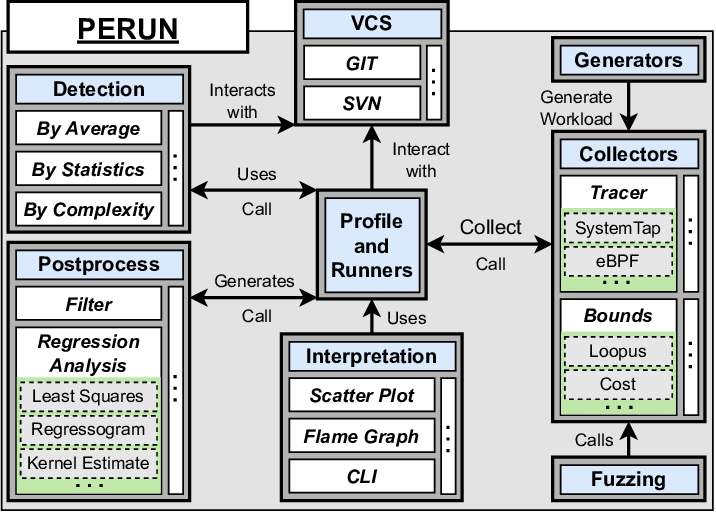
\includegraphics[width=4.5in]{obrazky-figures/perun-schema2.png}
    \caption{A schema of the Perun tool suite's architecture. \cite{perun-docs}}
    \label{fig:perun-schema}
\end{figure}

\section{Collectors}

Collectors measure a program's performance to create profiles. Their work can be divided into four phases:

\begin{itemize}
    \item \textbf{Before}: This is an optional phase that occurs before the actual collection of profiling data. Its purpose is to initialize the collector and prepare the project being profiled for the collection process, e.g., using a custom compilation process.
    \item \textbf{Collect}: In this phase, the profiled program is run, the collector collects the raw performance data, and, ideally, generates the profile in the unified format.
    \item \textbf{After}: The final and optional phase occurs after the resources have been successfully collected. This phase includes filtering or transforming the profile as needed.
    \item \textbf{Teardown}: In this phase, the collection resources are cleaned up. e.g., files, processes, locks, kernel modules, etc.
\end{itemize}

\noindent
Perun's API allows users to register their own collector by defining the \verb|before|, \verb|collect|, \verb|after| and \verb|teardown| methods in the collector's \verb|run.py| module. Additionally, Perun comes with several pre-registered collectors, focused on profiling various performance metrics. The profiling tool developed in this thesis will soon be on the list of available collectors.


\subsection{Time Collector}
As a simple wrapper over the Unix \verb|time| utility, this collector provides the total execution time of the program, as well as the amount of user time (the actual work of the program) and kernel time (the time spent executing system calls).

\subsection{Memory Collector}
This collector provides information about memory allocations in C/C++ programs. It logs the amount of allocated memory, allocation type (e.g., \texttt{malloc}, \texttt{realloc}), address of the allocated memory, and the location in the source code where the allocation took place, together with the stack trace at the time of allocation. It accomplishes this by overriding the standard C library's memory allocation functions with custom functions, which log the additional information and delegate the allocation to the original functions. \cite{memory-collector}


\subsection{Complexity Collector}
This collector gathers information about time spent in functions and the size of their inputs. It uses this information together with regression analysis to estimate the complexity of algorithms. It is based on compile-time instrumentation through the \texttt{-finstrument-functions} command line parameter of the \texttt{gcc} and \texttt{clang} compilers. \cite{complexity-collector}

\subsection{Trace Collector}
Trace collector (Tracer) is the most sophisticated collector that comes with Perun. It measures time spent in functions of C and C++ programs by collecting timestamps at the entry and exit points of functions. It is built on \emph{SystemTap} and \emph{eBPF} frameworks, thus relying on binary instrumentation. It is extendable, allowing new profiling frameworks to be integrated into Tracer, and there is currently a pending merge request\footnote{PIN-based Tracer engine with visualizations: \url{https://github.com/Perfexionists/perun/pull/157/commits}} in the Perun repository for a new Tracer engine\footnote{Tracer engine \,--\, the underlying framework that performs the instrumentation.} that uses Intel Pin as the underlying framework. Tracer is highly configurable, allowing users to select, e.g., the instrumentation engine, the probing strategy (which can be set to utilize sampling), or manually specify the functions to be profiled. If no functions are specified, Tracer can automatically extract the functions from the binary based on the selected probing strategy. Figure \ref{fig:tracer-schema} shows Tracer's profiling workflow. 


\begin{figure}[t]
    \centering
    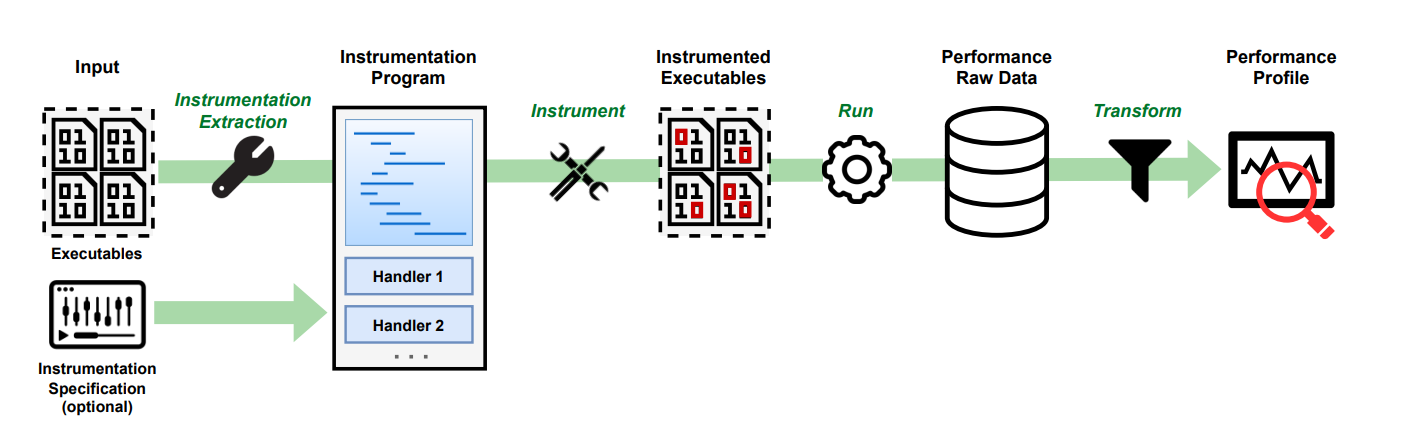
\includegraphics[width=6in]{obrazky-figures/Tracer-workflow.png}
    \caption{Schematic representation of Trace collector's workflow. \cite{perun-paper}}
    \label{fig:tracer-schema}
\end{figure}


Collecting the time spent in a program's functions is a resource-intensive endeavor, especially if the user requires a complete picture of the program's performance and, therefore, does not consider sampling as a viable method of reducing the profiling overhead. Additionally, Tracer's underlying frameworks are based exclusively on dynamic binary instrumentation, which, as described in Chapter \ref{performance-analysis}, generally incurs higher time overhead than other types of instrumentation. The engines currently supported by Tracer are only built for the Linux platform, compromising Tracer's flexibility and applicability across different operating systems. The \emph{SystemTap} engine also requires the user to install a compatible kernel version with debugging symbols, which places a heavy prerequisite burden on the user. This requirement can be a significant barrier for users who do not have the necessary permissions or capabilities to change their system's kernel, such as users using managed or restricted environments where such modifications are not permitted.

The new collector developed in this thesis aims to address these shortcomings by providing the option to measure cheaper metrics, utilizing compile-time instrumentation, and offering a less restrictive set of dependencies.



\chapter{LLVM Compiler Infrastructure}
\label{llvm}

LLVM is a modern, modular, open-source compiler infrastructure, built around a source-independent intermediate representation LLVM IR. It is primarily used to compile languages from the C language family, e.g., C, C++, or Objective C. The modular nature of the compiler allows for other languages to be compiled as well, provided that there is a front-end that can compile the language in question into the aforementioned LLVM IR language. Therefore, many compilers for other programming languages leverage the LLVM infrastructure for optimizations and machine code generation, e.g., \emph{swiftc}, the compiler for the \emph{Swift} programming language, or the \emph{Glasgow Haskell Compiler}. \cite{swift-docs, haskell-docs}

This chapter describes LLVM's architecture, LLVM IR, and the Pass Framework, which can be used to customize the compilation process. The information included in this chapter is based primarily on the online LLVM API documentation, the LLVM language reference manual, and the LLVM conference paper. \cite{llvm-api, llvm-lang-ref, llvm-paper}
\section{Architecture}

\begin{figure}
    \centering
    \includesvg[width=6in]{obrazky-figures/llvm-arch.svg}
    \caption{A High-level overview of LLVM's three-phase architecture. The front end for a given source language compiles the source code to LLVM IR, which acts as input to the optimizer. After optimizations, the target architecture is selected, and the appropriate backend generates object code or assembly code for the selected architecture. \cite{architecture-of-os-applications}}
    \label{fig:llvm-arch}
\end{figure}

The LLVM infrastructure comprises several sub-projects that work together to provide a comprehensive compiler framework. Its architecture is based on the popular three-phase architecture on which many modern compilers are built \cite{architecture-of-os-applications}. The first part is the front end, responsible for parsing the source code and creating an intermediate representation. Then comes the middle end, which analyses the intermediate representation and performs optimizations. Lastly comes the back end, which takes the optimized intermediate representation and turns it into the target architecture's machine or assembly code. LLVM's modular nature allows for each of these parts to be swapped out, meaning that compiler developers can create a front end for any programming language and use the other parts of the LLVM infrastructure for optimizations and target code generation. The same applies to the back end \,--\, languages with an implemented front end to LLVM IR can be ported to new architectures by creating a new back-end module that compiles LLVM IR into that architecture's instruction set. Figure \ref{fig:llvm-arch} shows a high-level schema of LLVM's architecture.

\section{LLVM IR}

Using an intermediate representation in the compilation process simplifies the compiler optimizations that make the resulting machine code more efficient. LLVM uses a custom intermediate representation called LLVM IR. It is designed to be a source-language-agnostic representation, allowing all kinds of languages to be compiled into this common representation and leverage the possibilities of the entire LLVM toolchain. LLVM IR is based on the SSA (Single Static Assignment) form, which dicatates that every variable is a target of only one assignment and the definition of a variable dominates all of its uses. This form simplifies and improves the efficiency of several types of optimizations, including constant propagation, value numbering, or partial-redundancy elimination. \cite{advanced-compiler-design}

LLVM IR is designed to be used in three equivalent forms: an in-memory compiler IR, an on-disk bitcode representation to be used for JIT compilers, and a human-readable representation useful for debugging purposes.

LLVM programs are composed of \emph{Modules}, with one module created for every compilation unit in the source code. Modules can also be linked using the \emph{llvm-link} tool provided by the toolchain.


\begin{figure}[h!]
    \centering
    \begin{minipage}[t]{0.45\textwidth}
            \begin{lstlisting}[language=c, caption={A module written in the C language, containing one function and one global variable.}, label={lst:ccode}]
            
int global_variable = 0;
int main() {
    int local_variable = 5;
    global_variable = 10 + local_variable;
    return 0;
}
        \end{lstlisting}
        \begin{lstlisting}[language=llvm, caption={Location nodes in the LLVM metadata graph. The nodes are prefixed with the \texttt{!} character and they are being referenced from the IR instructions.}, label={lst:llvm-metadata}]
!3 = !DIFile(filename: "main.c", ...)
!14 = distinct !DISubprogram(...)
!18 = !DILocalVariable(name: "local_variable", ...)
!19 = !DILocation(line: 4, column: 6, scope: !14)
!20 = !DILocation(line: 5, column: 9, scope: !14)
!21 = !DILocation(line: 5, column: 24, scope: !14)
!22 = !DILocation(line: 5, column: 2, scope: !14)

        \end{lstlisting}
    \end{minipage}%
    \hfill
    \begin{minipage}[t]{0.5\textwidth}
        \begin{lstlisting}[language=llvm, caption={An LLVM IR module compiled from the code shown in listing \ref{lst:ccode}. Apart from regular instructions, it contains a debugger intrinsic instruction \texttt{llvm.dbg.declare}, which tracks a source code variable through compiler optimizations.}, label={lst:llvm-ir}, aboveskip=3mm]
        
; ModuleID = 'main.c'
source_filename = "main.c"
target triple = "x86_64-unknown-linux-gnu"

@global_variable = dso_local global i32 0, align 4, !dbg !0

; Function Attrs: noinline nounwind optnone uwtable
define dso_local i32 @main() #0 !dbg !14 {
  %1 = alloca i32, align 4
  %2 = alloca i32, align 4
  store i32 0, ptr %1, align 4
  call void @llvm.dbg.declare(metadata ptr %2, metadata !18, metadata !DIExpression()), !dbg !19
  store i32 10, ptr %2, align 4, !dbg !19
  %3 = load i32, ptr %2, align 4, !dbg !20
  %4 = add nsw i32 %3, 5, !dbg !21
  ret i32 %4, !dbg !22
}
        \end{lstlisting}
    \end{minipage}
    \label{fig:c-and-llvm-ir}
\end{figure}

\subsection{LLVM IR Module}

LLVM IR modules contain global variables, type definitions, target architecture metadata, function declarations, and definitions. Optionally, debugging information in a debugger-agnostic format may be included as well. This format is convertible to different formats to be consumed by various debuggers (e.g. DWARF format for DWARF-based debuggers or a proprietary format such as PDB for Microsoft Visual Studio debugger).

Listing \ref{lst:llvm-ir} shows the LLVM IR module produced by \emph{clang} by compiling C code shown in Listing \ref{lst:ccode}



\subsubsection{Identifiers}

LLVM identifiers are either global or local. A global identifier is prefixed with the \texttt{@} character, while local identifiers, primarily virtual registers, are prefixed with the \texttt{\%} character. Values can be named or unnamed: named values are identified by their scope prefix and a string, which corresponds to their name in the original source code. Unnamed values are identified by their scope prefix and an integer.


\subsubsection{Functions}
Functions in LLVM modules can be either defined with complete bodies or declared as external references. Each function is linked to an attribute node that specifies its characteristics, such as calling conventions or optimization strategies.

Functions consist of basic blocks\footnote{Basic block \,--\, a linear sequence of instructions that has one entry point and one exit point.}, each uniquely identified within the scope of its function. By default, basic blocks are labeled with integer identifiers, which share the integer pool with virtual registers in the same function. However, the \texttt{clang} compiler option \texttt{fno-discard-value-names} can be used to give basic blocks more descriptive labels depending on their relationship to the source code. For example, a basic block that represents an else block in a conditional structure is named \texttt{if.else}.


\subsubsection{Instructions}
Basic blocks are comprised of instructions. Most LLVM IR instructions are in 3-address form, meaning they take one or two inputs, produce a single result, and store this result in the destination operand. The instruction set was designed to be a low-level representation of a program, thus enabling a straightforward compilation to target architectures while supporting high-level analyses and transformations. Apart from arithmetic, bitwise, and memory access operations, which are standard in all 3-address languages, LLVM IR contains many other types of instructions, such as vector instructions which represent vector operations in a target-independent way, or $\phi$-instructions, which select the correct value for variables depending on which path was taken through the control flow. \cite{llvm-ir-set}



\subsubsection{Metadata}

At the end of each LLVM IR module are debugging metadata. Metadata nodes are prefixed with the \texttt{!} character and contain different types of information depending on the node type, such as information about data types, information about which lines in the source code created a particular instruction, and others. The identifiers of metadata nodes are attached to IR instructions, and some types of nodes can contain links to other nodes, forming a graph. Listing \ref{lst:llvm-metadata} contains some metadata nodes, which are attached to instructions in Listing \ref{lst:llvm-ir}.


\section{LLVM Pass Framework}

LLVM \emph{Passes} are modular components within the LLVM framework designed to analyze or transform the LLVM IR of programs during compilation. They are primarily used to facilitate compiler optimizations or to gather additional debugging information about the program. Passes operate at various granularities, defined by the \emph{unit} of IR on which the pass operates, e.g., a loop, a function, or an entire module. Passes are grouped into \emph{pass pipelines} that define which passes are run on each unit of IR and in what order \,--\, for example, depending on the chosen optimization level using the \verb|-O| parameter in \texttt{clang}, a different pass pipeline is internally constructed and run on the program.

LLVM's C++ API allows developers to create their own passes, allowing for custom analyses and transformations. These passes can be created as standalone executable programs linked with the LLVM API, or as \emph{Pass Plugins}, which are executed after being loaded into other LLVM tools as shared objects.

\subsubsection{Relevant classes}
Before a Pass can be executed on a unit of IR, several classes have to be instantiated. These classes include the \texttt{PassBuilder} and the \texttt{PassManager}\footnote{There are currently two pass managers in the LLVM project: a new pass manager, introduced in LLVM 13, and the legacy pass manager. In this thesis, the term `pass manager' refers to the new pass manager. While the legacy pass manager is still available in recent LLVM versions, it is now considered deprecated and will eventually be removed.}, which facilitate the building and running of the pass pipelines, and a specific instance of an \texttt{AnalysisManager} class (e.g., a \texttt{ModuleAnalysisManager} for Module Passes).
A \texttt{PassManager} contains a sequence of passes, which run one after another on a unit of IR. The pass manager itself is a pass responsible for running the passes it contains and propagating the \texttt{AnalysisManager} object to the passes it runs.

The \texttt{AnalysisManager} object caches the computed analyses of each pass in the pipeline, allowing for faster pipeline executions without performing redundant analyses. To accomplish this, the \texttt{run()} method of a pass returns a \texttt{PreservedAnalysis} object, which contains the analyses that are preserved after the pass finishes running. Passes that do not transform the IR in any way (referred to as \emph{Analysis passes}) typically return the \texttt{PreservedAnalyses::all()} object, which tells the next pass in the pipeline that no previously computed analyses have been invalidated. Passes that modify the IR (referred to as Transformation Passes) typically invalidate the results of many previous analyses and must either return the \texttt{PreservedAnalyses::none()} object, which invalidates all previously computed analyses, or the programmer can build a custom \texttt{PreservedAnalyses} object and add a set of analyses which are preserved and can be used by the following passes.

Passes extend the \texttt{PassInfoMixin} class. They override the \texttt{run()} method, which takes an instance of \texttt{AnalysisManager} and the reference to the unit of IR the pass is supposed to operate on. The Pass Manager enables the registration of four types of passes, depending on the unit:

\begin{itemize}
    \item Module Pass \,--\, runs on an entire LLVM IR module.
    \item CGSCC (Call-Graph Strongly Connected Components) Pass \,--\, runs on strongly connected components in the call graph, typically used for callee simplification and inlining passes.
    \item Function Pass \,--\, runs on one function in a module at a time, independent of other functions in the module.
    \item Loop Pass \,--\, runs on every loop inside a function, independent of other loops in the function.
\end{itemize}


This pass hierarchy exists primarily for the purposes of pipeline optimization. Declaring a pass as, e.g., a Function Pass does not restrict its ability to modify the containing module. However, separate invocations of the same pass are completely independent and do not share any internal state. For this reason, even if a pass needs to modify only the bodies of individual functions but requires information about other functions to perform these modifications, it makes sense to use a Module Pass. Doing the same with a Function Pass would require managing the state through external means, such as by writing to and reading from files.


\subsection{Pass Plugins}
Pass plugins are LLVM passes that are injected into the compiler's default optimization pipelines. This is achieved by registering the custom pass with the \texttt{PassManager} object and using the \texttt{PassBuilder} object to specify the point in the optimization pipeline where the custom pass should run, e.g., after or before loop-related optimizations. Plugins are designed to be loaded into compatible LLVM tools, such as \texttt{clang} or \texttt{opt}. To make them recognize passes as valid plugins, at least one of two entry points has to be provided by the plugin.

\begin{itemize}
    \item \textbf{Static entry point}. This entry point is used in case the developer wants to link the plugin with compatible tools statically. This makes sense, for example, when developing a pass directly in the LLVM source tree with the goal of contributing to the project.
    \item \textbf{Dynamic entry point}. This entry point is used when the pass plugin is compiled into a shared library, which can be loaded into compatible tools through command line options. 
\end{itemize}

In either case, the entry point is a function that returns an instance of the  \texttt{PassPlugin\-LibraryInfo} structure. This structure provides the necessary information to the tool running this pass. Specifically, it contains the LLVM API version that the plugin understands, the name and version of the plugin, and a callback function that registers the pass with the \texttt{PassBuilder} instance of the tool that loaded this plugin. Listing \ref{lst:samplepass} contains an example of a simple pass plugin that runs on the Module unit and contains both a static and a dynamic entry point.

\begin{figure}[t]
    \centering
    \begin{lstlisting}[language=C++, caption={An example of a simple analysis LLVM Pass Plugin, operating on the Module unit. The pass prints the name of the module to the standard error output stream. The functions \texttt{getSamplePassPluginInfo()} and \texttt{llvmGetSamplePassPluginInfo()} act as the static and dynamic entry point for plugin-compatible LLVM tools.}, label={lst:samplepass}]
using namespace llvm;
class SamplePass : public PassInfoMixin<SamplePass> {
    public:
        // This function is called by the PassManager to run the pass.
        PreservedAnalyses run(Module &M, ModuleAnalysisManager &MAM) {
            errs() << M.getName() << "\n";
            return PreservedAnalyses::all();
        }
};

// Entry point for the static registration of the plugin
PassPluginLibraryInfo getSamplePassPluginInfo() {
    auto passPluginCallback = [](PassBuilder &PB) {
        // Registers the pass at the end of the function
        // optimization pipeline
        PB.registerOptimizerLastEPCallback(
                [](ModulePassManager &MPM, OptimizationLevel L) {
                    MPM.addPass(SamplePass());
                }
        );
    };
    return {LLVM_PLUGIN_API_VERSION, "sample-pass", "v1.0", passPluginCallback};
}

// Entry point for the dynamic registration of the plugin
extern "C" 
PassPluginLibraryInfo LLVM_ATTRIBUTE_WEAK llvmGetSamplePassPluginInfo() {
    return getSamplePassPluginInfo();
}
    \end{lstlisting}
\end{figure}




\section{Instrumentation in LLVM}
While the IR generation capabilities of the LLVM API are primarily intended for developing new language front-ends, the same API can also be used to perform custom instrumentation. The simplest and most efficient way to build new instructions is through the \texttt{IRBuilder} class, which provides methods for creating all types of instructions and inserting them into basic blocks. The user can specify an insertion point to the \texttt{IRBuilder} through its \texttt{SetInsertionPoint()} method, which takes an instance of \texttt{Instruction} as a parameter. Any instructions created through that instance of \texttt{IRBuilder} will be placed before the instruction set as an insertion point. Besides instructions, the \texttt{IRBuilder} can insert new global variables into the module or create and modify metadata.

Instrumentation will typically involve inserting call instructions, which call instrumentation functions located in a separate instrumentation code module. Before a call can be inserted, the function first has to be declared inside the module. This can be easily done through the \texttt{Module} object's \texttt{getOrInsertFunction()} method, which takes the name of the function and a \texttt{FunctionType} object that contains the signature of that function. The method returns a \texttt{FunctionCallee} object, which is passed to the \texttt{IRBuilder}'s \texttt{CreateCall()} method together with the arguments in the form of instances of the \texttt{Value} class. These instances can also be created with the \texttt{IRBuilder}, which provides methods such as \texttt{getInt32()} that take an integer value as input and return a \texttt{ConstantInt} object which represents that value in LLVM IR. 


\chapter{Design and Implementation}
\label{implementation}

As stated in previous chapters, this work aims to leverage the LLVM Pass Framework API to implement a lightweight profiler based on compile-time static instrumentation. This chapter describes the optimizations performed in different versions of this profiler and the core design philosophy and implementation details. Section \ref{benchmarks} introduces the benchmarks on which we evaluate the performance of each new profiler version. Sections \ref{hashtable-impl}, \ref{onearray}, \ref{multiarray}, and \ref{patterns} describe the changes between major optimized versions of the profiler, and their performance is compared using the benchmarks.

\section{Benchmarks}
\label{benchmarks}

The profiler was benchmarked on one small C project and one larger C project to evaluate its efficiency. The smaller project is a program implementing the CCSDS compression algorithm\footnote{\url{https://pajda.fit.vutbr.cz/perferts/ccsds}} used to compress images taken on a spacecraft before sending them to Earth. The larger project is \texttt{CPython}\footnote{CPython GitHub repository: \url{https://github.com/python/cpython}}, the reference implementation of the Python programming language and the most widely used Python interpreter. 

The estimated profiling overhead on the CCSDS project was obtained by running the compression algorithm on different input images\footnote{\url{https://pajda.fit.vutbr.cz/perferts/ccsds-data}}. The original and instrumented versions of the compiled executable ran 100 times; the average runtime was calculated for each input, and these two averages were compared. Table \ref{tab:ccsds-img} shows the information about images used as inputs.

\begin{table}[t]
    \centering
    \begin{tabular}{lrrrr}
    \textbf{Image} & \textbf{Width} & \textbf{Height} & \textbf{Max gray value} & \textbf{Size} \\
    \hline 
    \hline
    cdf97-psi.pgm & 609 & 423 & 255 & 257 KB \\
    Babboon.pgm & 512 & 512 & 255 & 262 KB \\
    P1010042.pgm & 591 & 591 & 255 &  349 KB \\
    frame.pgm & 1920 & 1080 & 65535 & 4.15 MB \\
    g10.pgm & 3840 & 2160 & 1023 & 16.59 MB \\
    m612-be.pgm & 2564 & 5117 & 4095 & 26.24 MB \\
    \end{tabular}
    \caption{Input images for CCSDS benchmarks}
    \label{tab:ccsds-img}
\end{table}


For CPython benchmarks, the Python package PyPerformance \cite{pyperformance} was used to evaluate performance. PyPerformance is a project that aims to evaluate the interpreter's performance in various benchmarks, from testing templating libraries or serialization to math operations and raytracing. A subset of PyPerformance benchmark groups were selected for the experimental evaluation:

\begin{itemize}
    \item {\textbf{MATH}: Set of benchmarks focused on testing the performance of big integer arithmetic and floating point number calculations.}
    \item {\textbf{REGEX}: Several benchmarks testing the performance of Python's regular expression engine.}
    \item {\textbf{SCIMARK}: A popular set of benchmarks for scientific and mathematical computing, including Fast Fourier Transform, Monte Carlo algorithm, or sparse matrix multiplication.}
    \item {\textbf{APPS}: A benchmark testing several application libraries, such as the Tornado HTTP web framework or the Chameleon templating engine.}
    \item {\textbf{SERIALIZE}: A larger group of serialization and de-serialization benchmarks, testing the JSON and pickle modules.}
\end{itemize}

Table \ref{tab:cpython-benchmarks} shows the PyPerformance benchmarks contained in each group.

\begin{table}[]
    \renewcommand{\arraystretch}{1.5}
    \centering
    \begin{tabular}{m{5cm}m{10cm}}
    \textbf{Benchmark group} & \textbf{Benchmarks} \\ 
    \hline
    \hline
    Math & \begin{myverbbox}[\small]{\vmath}nbody, pidigits, float
\end{myverbbox}
\vmath \\ \hline
    Regex & \begin{myverbbox}[\small]{\vregex}regex_compile, regex_dna, regex_effbot, regex_v8
\end{myverbbox}
\vregex \\ \hline
    Scimark & \vspace{3pt}\begin{myverbbox}[\small]{\vscimark}scimark_fft, scimark_lu, scimark_monte_carlo,
scimark_sor, scimark_sparse_mat_mult
\end{myverbbox}
\vscimark \\ \hline
    Apps & \begin{myverbbox}[\small]{\vscimark}2to3, chameleon, docutils, html5lib, tornado_http
\end{myverbbox}
\vscimark \\ \hline
    Serialize & \vspace{3pt}\begin{myverbbox}[\small]{\vserialize}json_dumps, json_loads, pickle, pickle_dict,
pickle_list, pickle_pure_python, tomli_loads,
unpickle, unpickle_list, unpickle_pure_python,
xml_etree
\end{myverbbox}
\vserialize \\ \hline
    \end{tabular}
    \caption{PyPerformance benchmark groups used in the evaluation and the specific benchmarks they contain.}
    \label{tab:cpython-benchmarks}
\end{table}


All benchmarks were run on a machine with the following specifications:

\begin{table}[H]
    \centering
    \begin{tabular}{ll}
    \textbf{CPU} & AMD Ryzen 5 3500U \\
    \textbf{Memory} & 16GB @ 2666 MHz \\
    \textbf{OS} & Linux Mint 20.3 Cinnamon \\
    \textbf{Kernel version} & 5.13.0-52-generic\\
    \end{tabular}
    \label{tab:ccsds-images}
\end{table}

\section{Hashtable-based implementation}
\label{hashtable-impl}

In this first version of the profiler, the \verb|std::unordered_map| class from the standard C++ library was used to store information about the number of executions of each basic block. This unordered map uses a unique identifier of each basic block as a key and stores a corresponding execution count as the value. The key contains the name of the basic block and the name of the function and module it belongs to. The map is declared in the instrumentation code module, which is linked to the instrumented program after the compilation. A call to an instrumentation function \texttt{\_\_bb\_enter()} is inserted at the start of every basic block. This function takes the unique identifier of the basic block as input, checks if this identifier is already present in the map, and either increments the existing counter or creates a new key-value pair for this basic block. To export the collected data, a call to a function \texttt{\_\_prof\_export()}, which writes the resulting profile into a file, is inserted before the return instruction from the \texttt{main()} function and also before every call to the \texttt{exit()} function.

This approach is very simple and convenient, as no additional processing has to be done besides the instrumentation. Additional information about the basic blocks, such as the source code location, can be included directly in the identifier saved in the map, creating almost no compilation overhead. This approach also guarantees that memory is allocated only for basic blocks that were executed at least once\footnote{Excluding the memory that is pre-allocated automatically by all standard library containers to reduce the number of re-allocations.}, minimizing the memory overhead compared to a structure that would statically allocate space for every basic block in the program.

However, even though the map has a constant time complexity for searching and inserting, the added runtime overhead of this approach is extremely high. To keep the time complexity constant on average, the map has to periodically allocate space for new buckets to accommodate additional basic blocks. This frequent reallocation can be very expensive, potentially explaining the massive overhead. Additionally, the hash function could be very expensive, causing further time overhead. Table \ref{tab:hashtable-ccsds} shows the measured overhead of this implementation on the CCSDS project. Because the overhead on a smaller project was already so large, this version was not tested on \texttt{CPython}, as it would easily exceed the one-hour timeout limit which was used with these benchmarks.


\begin{table}[]
    \centering
    \begin{tabular}{lrrr}
    \textbf{Image} & \textbf{Original time [s]} & \textbf{Instrumented time [s]} & \textbf{Overhead}  \\ 
    \hline
    \hline
    cdf97-psi.pgm & 0.029 & 1.646 & 56.76x \\
    Babboon.pgm & 0.030 & 1.627 & 54.23x \\
    P1010042.pgm & 0.039 & 2.177 & 55.82x \\
    frame.pgm & 0.279 & 15.075 & 54.03x \\
    g10.pgm & 0.815 & 38.879 & 47.70x \\
    m612-be.pgm & 1.431 & 70.762 & 49.45x \\ \hline
    Average & & & 52.99x
    \end{tabular}
    \caption{The profiling overhead measured on CCSDS of a hashtable-based implementation.}
    \label{tab:hashtable-ccsds}
\end{table}



\section{An array-based implementation}
\label{onearray}
To prevent the overhead caused by frequent hashing using an expensive hash function and frequent memory reallocations, a static array can be used to store the basic block execution counts. Indexing an array also has a constant time complexity, and if the array is statically allocated, no runtime memory reallocation is required.

 The array is declared as a static global array of unsigned long integers in the instrumentation code module, and the \texttt{\_\_bb\_enter()} function is used to increment the values inside this array. As with the previous implementation, a call to this function is inserted at the start of every basic block. Each basic block is assigned an unsigned long integer ID. This ID is used as an index into this execution count array. Before the program exits, the execution counts are exported in a simple format, mapping the ID of the basic block to the number of its executions.

This approach, however, requires additional processing during compile time. Since only the ID and execution count of each basic block are exported after profiling, the other information about the basic blocks has to be exported during compile time. Post-processing is also necessary to map the IDs to the basic block information.
To ensure that the array can accommodate all basic block execution counters, the instrumentation code must be compiled with a macro definition containing the number of basic blocks in the profiled program, passed to the compiler with the \texttt{-D} command line option. This means that the instrumentation code has to be compiled specifically for every program.

\begin{table}[]
    \centering
    \begin{tabular}{lrrr}
    \textbf{Image} & \textbf{Orig. time [s]} & \textbf{Inst. time [s]} & \textbf{Overhead}  \\ 
    \hline
    \hline
    cdf97-psi.pgm &  0.029 & 0.069 & 2.38x \\
    Babboon.pgm & 0.030 & 0.064 & 2.13x \\
    P1010042.pgm & 0.039 & 0.087 & 2.23x \\
    frame.pgm & 0.279 & 0.659 & 2.36x \\
    g10.pgm & 0.815 & 1.700 & 2.08x \\
    m612-be.pgm & 1.431 & 3.153 & 2.20x \\ \hline
    Average & & & 2.23x
    \end{tabular}
    \caption{The profiling overhead measured on CCSDS of an implementation using a single static array to store execution counts.}
    \label{tab:single-array-ccsds}
\end{table}

While this approach sacrifices the memory efficiency of only allocating memory for basic blocks that were executed at least once, the time overhead is significantly reduced. Table \ref{tab:single-array-ccsds} shows the measured overhead of this implementation on the CCSDS project. This implementation was tested on the CPython project as well, but all of the PyPerformance benchmark runs have timed out after 1 hour. This shows that while there is a significant performance improvement over the previous implementation, the solution still does not scale well.

Using a single array still has a major flaw, though. Since each basic block needs to have a unique ID assigned during compilation, the instrumentation pass has to keep track of the last assigned ID after instrumenting a module. As mentioned in Chapter \ref{llvm}, separate invocations of a pass do not share any internal state, which means that to remember the last assigned ID, it has to be written to a file after each invocation and then read back at the start of the next invocation. While this operation does not add significant overhead to compile time, it makes it impossible for multiple compilation jobs to be run concurrently, making this approach unsuitable for larger projects. This flaw is addressed in Section \ref{multiarray}.

\section{Inlining instrumentation code}
\label{inlining}
Inline expansion (inlining) refers to replacing a function call with the function's body, eliminating the call instruction and the overhead associated with it. This includes saving the register content from the caller's context, passing the function parameters, and creating a stack frame. Inlining is typically performed automatically by the compiler, which can decide to inline a function at only a subset of call sites, using heuristics to determine where such an expansion is likely to affect performance positively. According to \cite{advanced-compiler-design}, these heuristics take into account the following:

\begin{enumerate}
    \item The size of the function's body: the smaller, the better.
    \item The number of calls to the function: with only one call, inlining is almost certain to reduce execution time.
    \item Whether the function is called inside a loop: if so, inlining it could provide opportunities for additional optimization.
    \item Whether the call includes constant-valued parameters, which makes it more likely that the inlined body of the function is optimizable.
\end{enumerate}

Since the body of the  \verb|__bb_enter()| function contains only code that indexes an array and increments an integer, and its only argument is the constant ID of the basic block, points 1 and 4 are relevant. The overhead associated with setting up the function call could be relatively high compared to the actual work of the function. Inlining could also improve the locality of reference, providing further performance improvement by reducing the number of cache misses. \cite{inline-func} However, because the instrumentation function is defined in the instrumentation code module, but called from the modules of the profiled program, the compiler cannot inline this call automatically without using link-time optimization, which is a feature that is not by default supported by most compilers. Therefore, the instrumentation function was removed and instead of inserting a function call, the instrumentation pass inserts a \verb|load| instruction to read the current count for that basic block from memory, the \verb|add| instruction to increment the counter, and the \verb|store| instruction to write back the updated counter. 

The result of this optimization can be observed in the \verb|objdump| output of the instrumented binary. Listing \ref{lst:instrumented-callq} shows the disassembled contents of the \texttt{bio\_get\_bit()} function, instrumented with calls to \texttt{\_\_bb\_enter()}. Listing \ref{lst:instrumented-inline} shows the same function with inline instrumentation. Listing \ref{lst:bbenter-objdump} shows the body of the \texttt{\_\_bb\_enter()} function.

\lstset{
  language=x86asm,
  basicstyle=\ttfamily\small,
  backgroundcolor=\color{gray!10},
  frame=single,
  breaklines=true,
  captionpos=b,
}


\begin{figure}[t]
    \centering
    \begin{minipage}[t]{.48\textwidth}  % Left side
        \centering
        \begin{lstlisting}[caption={Disassembled object code of the \texttt{\_\_bb\_enter()} function.}, label={lst:bbenter-objdump}]
0000000000001b10  <__bb_enter>:
  mov    0x1691(%rip),%rax # 31a8 <_DYNAMIC+0x1d8>
  mov    (%rax,%rdi,8),%rcx
  add    $0x1,%rcx
  mov    %rcx,(%rax,%rdi,8)
  retq  
        \end{lstlisting}

        \begin{lstlisting}[caption={Disassembled code of a part of the CCSDS \texttt{bio\_get\_bit()} function, instrumented inline with load, add, and store instructions. The \texttt{lea} instruction loads the address of the \texttt{\_\_basicblocks} array into the \texttt{\%rcx} register at the start of the function, after which the \texttt{incq} instruction records each basic block's execution.}, label={lst:instrumented-inline}]
0000000000214020 <bio_get_bit>:
  lea    0xb2a9(%rip), %rcx       # 21f2d0 <__basicblocks>
  incq   0x8580(%rcx)
  cmpq   $0x8,0x18(%rdi)
  jne    214064 <bio_get_bit+0x44>
  incq   0x8590(%rcx)
  mov    0x8(%rdi),%rax
  test   %rax,%rax
  je     21408b <bio_get_bit+0x6b>
  lea    0x1(%rax),%rdx
  incq   0x8598(%rcx)
  ...
        \end{lstlisting}
    \end{minipage}%
    \hfill
    \begin{minipage}[t]{.48\textwidth}  % Right side
        \centering
        \begin{lstlisting}[language={x86asm}, caption={Disassembled code of a part of the CCSDS \texttt{bio\_get\_bit()} function, instrumented with calls to \texttt{\_\_bb\_enter()}. The start of the function contains extra \texttt{push} instructions, as the caller has to save the contents of the registers. }, label={lst:instrumented-callq}, aboveskip=3mm]
0000000000412cd0 <bio_get_bit>:
  push   %rbp
  push   %r15
  push   %r14
  push   %rbx
  push   %rax
  mov    %rdi,%rbx
  mov    $0x251a,%edi
  mov    %rsi,%r14
  callq  41c6b0 <__bb_enter>
  cmpq   $0x8,0x18(%rbx)
  jne    412d25 <bio_get_bit+0x55>
  mov    $0x251c,%edi
  callq  41c6b0 <__bb_enter>
  mov    0x8(%rbx),%r15
  test   %r15,%r15
  je     412d4f <bio_get_bit+0x7f>
  mov    $0x251d,%edi
  callq  41c6b0 <__bb_enter>
  ...
        \end{lstlisting}
    \end{minipage}
\end{figure}


This optimization was very effective in reducing profiling overhead. Table \ref{tab:ccsds-inlined} shows the profiling overhead on the CCSDS project. Inlining the instrumentation code reduced the time overhead by 50\% on average, with the average overhead reduced to less than 10\%.

\begin{table}[]
    \centering
    \begin{tabular}{lrrr}
    \textbf{Image} & \textbf{Original time [s]} & \textbf{Instrumented time [s]} & \textbf{Overhead}  \\ 
    \hline
    \hline
    cdf97-psi.pgm & 0.029 & 0.030 & 1.03x \\
    Babboon.pgm & 0.028 & 0.031 & 1.11x \\
    P1010042.pgm & 0.038 & 0.041 & 1.08x \\
    frame.pgm & 0.254 & 0.288 & 1.13x \\
    g10.pgm & 0.768 & 0.842 & 1.10x \\
    m612-be.pgm & 1.339 & 1.485 & 1.11x \\ \hline
    Average & & & 1.09x
    \end{tabular}
    \caption{The profiling overhead measured on CCSDS with the instrumentation code inlined.}
    \label{tab:ccsds-inlined}
\end{table}

\section{A per-module static array implementation}
\label{multiarray}

As mentioned in Section \ref{onearray}, assigning each basic block in a program a unique ID restricts the ability to compile multiple modules concurrently, which would significantly affect the usability of this profiler on larger projects that take a long time to compile. To address this, each module of the program has a separate pool of integers to assign as IDs to its basic blocks, and rather than storing all execution counts in a single array, each module's basic block execution counts are stored in a separate array. Before the first basic block in each module is instrumented, a declaration of a pointer to unsigned long integer array is inserted into the module, with its linkage type set to external. The instrumentation pass keeps track of the number of basic blocks in the module. After the last one is instrumented, the name of the module, the name of the declared external pointer, and the number of basic blocks in the module are written to a temporary file  \texttt{modules.tmp}. Before linking the program, this file is consumed by another pass, called \texttt{PostInstrumentationPass}. This pass is designed to run on the instrumentation code module. It reads the \texttt{modules.tmp} file and defines the array variables inside the instrumentation code module. It also inserts one call to the function \texttt{\_\_export\_array()} per module, which exports the collected execution counts.

To relieve the user from the headache of setting up a custom compilation process, a simple shell script is provided to be used as a custom linker through clang's \texttt{-fuse-ld} command line option. This linker wrapper script automatically compiles the instrumentation code, runs the \texttt{PostInstrumentationPass}, and invokes the real linker with the original arguments plus the object file of the instrumentation code module.

\begin{table}[]
    \centering
    \begin{tabular}{lrrr}
    \textbf{Image} & \textbf{Orig. time [s]} & \textbf{Inst. time [s]} & \textbf{Overhead}  \\ 
    \hline
    \hline
    cdf97-psi.pgm & 0.029 & 0.033 & 1.14x \\
    Babboon.pgm & 0.028 & 0.033 & 1.18x \\
    P1010042.pgm & 0.038 & 0.043 & 1.13x \\
    frame.pgm & 0.254 & 0.309 & 1.22x \\
    g10.pgm & 0.768 & 0.894 & 1.16x \\
    m612-be.pgm & 1.339 & 1.543 & 1.15x \\ \hline
    Average & & & 1.16x
    \end{tabular}
    \caption{The profiling overhead measured on CCSDS with one counter array in each module.}
    \label{tab:ccsds-multi-array}
\end{table}

\begin{table}[]
    \centering
    \begin{tabular}{lrrr}
    \textbf{Benchmark} & \textbf{Orig. time [s]} & \textbf{Inst. time [s]} & \textbf{Overhead}  \\ 
    \hline
    \hline
    Math & 56.76 & 78.05 & 1.38x \\
    Regex & 95.59 & 111.03 & 1.16x \\
    Scimark & 122.58 & 151.03 & 1.23x \\
    Apps & 510.51 & 625.13 & 1.22x \\
    Serialize & 594.07 & 694.86 & 1.17x \\ \hline
    Average & & & 1.23x
    \end{tabular}
    \caption{The profiling overhead measured on an instrumented CPython interpreter running PyPerformance benchmarks, with one counter array in each module.}
    \label{tab:cpython-multi-array}
\end{table}


While the primary goal of this change was not to improve the profiler's overhead, it was still measured. This version of the profiler was also the first version that could successfully profile the CPython interpreter using the PyPerformance benchmarks. The overhead measurements on the CCSDS and CPython projects, as shown in Table \ref{tab:ccsds-multi-array} and Table \ref{tab:cpython-multi-array}, indicate that the changes described in this chapter may have slightly increased the overhead. However, the increase is not significant. For large projects, the ability to compile concurrently still accelerates the profiling process considerably.


\section{Control flow graph patterns}
\label{patterns}

In all previously described approaches, every basic block in the program was instrumented to obtain complete execution count information in the profiled program. However, by examining the control flow graph\footnote{A control flow graph is a directed graph $G = (B, E)$ in which the nodes ($B$) represent basic blocks and the edges ($E$) represent control flow paths. \cite{cfg-paper}} of each function before the instrumentation, some basic blocks could be excluded without sacrificing the completeness of the result. This is because the number of executions of a particular basic block could be inferred from the number of executions of another basic block, or a group of other basic blocks.

To test this approach, an algorithm to analyze the control flow graph of each function was developed. This algorithm checks for the presence of basic block patterns \,--\, subgraphs of the control flow graph \,--\, commonly observed in compiled programs as a result of high-level language control flow structures being compiled into a low-level language. 

For all formal definitions in this section, we define \(succ(x)\) as the set of immediate successors of a block \( x \), where \( y \) is an immediate successor of \( x \) if there is an edge from \( x \) to \( y \). Similarly, we define \(pred(x)\) as the set of immediate predecessors of a block \( x \), where \( y \) is an immediate predecessor of \( x \) if there is an edge from \( y \) to \( x \). Additionally, we define the function \(executions(b, in) : B \times I \to \mathbb{N}_0\), where \(B\) is the set of all basic blocks in a control flow graph \(G = (B, E)\) and \(I\) is the set of all possible inputs to the program. The function \(executions(b, in)\) represents the number of times the basic block \(b\) is executed by the program, given input \(in\).


\subsection{The Diamond pattern}

This pattern involves 4 or more basic blocks. It begins with an entry block, which then branches to any number of successors. These successors all have a single common successor. This common successor does not have any predecessors from outside this pattern. This pattern is typically generated from an if statement followed by an else statement. The entry block is the condition inside the if statement. This block branches into two blocks, which are executed depending on the boolean result of the if condition. Both blocks then join after the if-else statement. This pattern, with any number of branches, can also be compiled from a switch statement, though only the if-else statement support was implemented in this thesis.


\textbf{Formal definition.} Let \( G = (B, E) \) be a control flow graph. A \textbf{Diamond pattern} subgraph \( G' = (B', E') \) is defined as:
\begin{align}
    B' &= \{\text{entry}, b_1, b_2, \ldots, b_n, \text{join}\} \subseteq B, \\
    E' &= \{(\text{entry}, b_1), (\text{entry}, b_2), \ldots, (\text{entry}, b_n), (b_1, \text{join}), (b_2, \text{join}), \ldots, (b_n, \text{join})\} \subseteq E,
\end{align}
and the following conditions apply:
\begin{align}
succ(\text{entry}) &= \{b_1, b_2, \ldots, b_n\}, \\
\forall b_i \in \{b_1, b_2, \ldots, b_n\}:  
succ(b_i) &= \{\text{join}\} \land pred(b_i) = \{\text{entry}\}\\
pred(\text{join}) &= \{b_1, b_2, \ldots, b_n\}.
\end{align}


The entry and join blocks can be entirely excluded from the instrumentation. This is because the sum of the executions of the branch blocks will always equal the number of executions of the entry and join blocks as long as the program does not terminate in either of the branches. Formally, given an input \(in\),
\begin{align}
executions(\text{entry}, in) = executions(\text{join}, in) = \sum_{i=1}^{n} executions(b_i, in)
\end{align}
Figure \ref{fig:diamond-pattern} shows an example of a diamond pattern.

%\begin{figure}[t]
    %\centering
    %
\includegraphics[scale=0.5]{obrazky-figures/diamond.pdf}
    %\caption{Example of Diamond pattern in a control flow graph. The branch blocks, colored red, are instrumented, while the entry and end blocks are not.}
    %\label{fig:diamond-pattern}
%\end{figure}

\begin{figure}[h]
    \centering
      \begin{minipage}[t]{0.49\textwidth}
        \centering
        
\includegraphics[scale=0.75]{obrazky-figures/diamond.pdf}
        \caption{An example of the Diamond\\ pattern in a control flow graph. The\\ red blocks \texttt{if.then}, \texttt{if.else} are instru-\\mented, while the \texttt{entry} and \texttt{if.end} \\blocks are not.}
        \label{fig:diamond-pattern}
    \end{minipage}
    \begin{minipage}[t]{0.49\textwidth}
        \centering
        
\includegraphics[scale=0.75]{obrazky-figures/halfdiamond.pdf}
        \caption{An example of the Half-diamond pattern in a control flow graph. The \texttt{entry} block, colored blue, does not have to be instrumented, as its execution count can be inferred from the \texttt{if.end} block execution count.}
        \label{fig:halfdiamond-pattern}
    \end{minipage}%
    \hfill
\end{figure}



\subsection{The Half-diamond pattern}

This pattern is very similar to the diamond pattern, except the entry block has two successors, with one of these successors having a single edge, which leads to the other successor, who has no predecessor from outside this pattern. This pattern is often created by compiling an if statement not followed by an \verb|else| statement. The entry block is the if condition, the first successor is the block executed when the condition evaluates to true, and the other successor is the join block where the program continues regardless of whether the condition was evaluated as true or false.

\textbf{Formal definition.} Let \( G = (B, E) \) be a control flow graph. A \textbf{Half-diamond pattern} subgraph \( G' = (B', E') \) is defined as:
\begin{align}
    B' &= \{\text{entry}, b_1, \text{join}\} \subseteq B, \\
    E' &= \{(\text{entry}, b_1), (\text{entry}, \text{join}), (b_1, \text{join})\} \subseteq E, 
\end{align}
and the following conditions apply:
\begin{align}
    succ(\text{entry}) &= \{b_1, \text{join}\}, \\
    succ(b_1) &= \{\text{join}\}, \\
    pred(b_1) &= \{\text{entry}\}, \\
    pred(\text{join}) &= \{b_1, \text{entry}\}.
\end{align}


If this pattern is present in the control flow graph, either the entry block or the exit block can be excluded from the instrumentation, as the number of executions of one will always equal the number of executions of the other, as long as the program does not terminate inside the if-then block.
Formally, given an input \(in\)
\begin{align}
executions(\text{entry}, in) = executions(\text{join}, in)
\end{align}
Figure \ref{fig:halfdiamond-pattern} shows an example of this pattern.




\begin{wrapfigure}[17]{l}{0.5\textwidth} % Adjust the number of lines if necessary
  \centering
  
\includegraphics[width=0.5\textwidth]{obrazky-figures/uncond.pdf}
  \caption{Example of an unconditional jump in a control flow graph compiled from a for-loop. The \texttt{for.body} block can be excluded from instrumentation, as its number of executions will be identical to that of the \texttt{for.inc} block. }
  \label{fig:unconditional}
\end{wrapfigure}
\noindent
\subsection{Unconditional jump pattern}
This pattern contains two basic blocks. 
 The first basic block has a single edge to another basic block, and this successor has only the first basic block as a predecessor. Since an execution of the first block is always followed by an execution of the second block, only one of these blocks has to be instrumented.

\textbf{Formal definition.} Let \( G = (B, E) \) be a control flow graph. An \textbf{Unconditional jump pattern} subgraph \( G' = (B', E') \) is defined as:
\begin{align}
    B' &= \{b_1, b_2\} \subseteq B, \\
    E' &= \{(b_1, b_2)\} \subseteq E, \\
    succ(b_1) &= \{b_2\}, \\
    pred(b_2) &= \{b_1\}.
\end{align}

\medskip
Formally, given an input \(in\), the relationship between execution counts is
\begin{align}
executions(b_1, in) = executions(b_2, in)
\end{align}

This pattern primarily shows up in control flow graphs of functions containing for loops, as the \verb|clang| compiler sometimes separates the body and the increment part of the for loop into two basic blocks. However, compiler optimizations will likely remove any redundant unconditional jumps, meaning that this pattern is less likely to appear in practical scenarios. Figure \ref{fig:unconditional} shows an example of a control flow graph of a for loop that contains an unconditional jump.



\medskip\noindent
\subsection{Sum of exit block executions}

This pattern appears in every function containing more than one basic block. Since each function has a dedicated entry block with no incoming edges and any number of exit blocks, the entry block never has to be instrumented, as the sum of the number of executions of the exit blocks will equal the number of executions of the entry block, unless the program terminates before it reaches an exit block. 

\textbf{Formal definition}. Let \( G = (B, E) \) be a control flow graph. Define \(exits(G)\) as:
\begin{align}
exits(G) = \{ b \in B \mid \operatorname{succ}(b) = \emptyset \}
\end{align}
Define \(entry(G)\) as the block \( b\in B \) such that \(\operatorname{pred}(b) = \emptyset\). For a given input \(in\),
\begin{align}
\sum_{b \in exits(G)} executions(b, in) = \text{executions}(entry(G), in)
\end{align}


\begin{table}[]
    \centering
    {\small{\begin{tabular}{lrrrrrr}
    \multicolumn{1}{l}{\multirow{2}{*}{\textbf{Benchmark}}} & \multicolumn{1}{c}{\multirow{2}{*}{\textbf{Original [s]}}} & \multicolumn{2}{c}{\textbf{No pattern opt.}} & \multicolumn{2}{c}{\textbf{Pattern opt.}} & \multicolumn{1}{l}{\multirow{2}{*}{\textbf{Change [\%]}}} \\
    \cline{3-6} 
    \multicolumn{1}{l}{} & \multicolumn{1}{c}{} & \multicolumn{1}{c}{\textbf{Time [s]}} & \multicolumn{1}{c}{\textbf{Overhead}} & \multicolumn{1}{c}{\textbf{Time [s]}} & \multicolumn{1}{c}{\textbf{Overhead}} \\ 
    \hline
    \hline
    Math & 56.76 & 78.05 & 1.38x & 74.97 & 1.32x & 4.35\\
    Regex & 95.59 & 111.03 & 1.16x  & 110.18 & 1.15x & 0.86 \\
    Scimark & 122.58  & 151.03 & 1.23x & 149.66 & 1.22x & 0.81 \\
    Apps & 510.51 & 625.13 & 1.22x & 604.03 & 1.18x & 3.28 \\
    Serialize & 594.07 & 694.86 & 1.17x & 699.96 & 1.18x & -0.85 \\
    \hline
    \multicolumn{1}{l}{Average} & & & 1.23x & & 1.21x & 1.69 \\
    \end{tabular}
    }}
    \caption{A comparison of profiling overhead when using pattern optimizations vs no pattern optimizations on an instrumented CPython executable compiled with \texttt{-O3,} running PyPerformance benchmarks.}
    \label{tab:cpython-patterns}
\end{table}

\subsection{Impact of pattern optimizations on overhead}

Table \ref{tab:num-patterns} shows the number of patterns (excluding the \emph{sum of exits} pattern) found in CCSDS and CPython compiled with different optimization levels. The results show that the number of patterns found in unoptimized code is significantly higher than in optimized code. Tables \ref{tab:ccsds-patterns} and \ref{tab:cpython-patterns} show the impact of this optimization on the profiling overhead on the CCSDS and CPython benchmarks with compiler optimization level \texttt{-O3}.
Table \ref{tab:cpython-patterns-O0} shows the same for CPython compiled with \texttt{-O0}. While experiments on unoptimized programs have shown that it is a potentially viable method of reducing overhead, the impact of this optimization greatly diminishes when used together with compiler optimizations, while the impact on the compilation time is significant, as shown by Table \ref{tab:compilation-overhead}. Optimizing the pattern-finding algorithm or extending it with more complex patterns, which appear more often in compiler-optimized control flow graphs, could be a subject of future work.

\begin{table}[]
    \centering
    {\small
    \begin{tabular}{lrrr}
        \multirow{2}{*}{\textbf{Project}} & \multirow{2}{*}{\textbf{Original compilation time [s]}} & \multicolumn{2}{c}{\textbf{Compilation time with instrumentation [s]}} \\
        \cline{3-4}
         & & \textbf{No pattern opt.} & \textbf{Pattern opt.} \\
         \hline
         \hline
         CCSDS & 2.708 & 3.207 & 4.159 \\
         CPython & 24.581 & 76.499 & 435.14 \\
    \end{tabular}
    }
    \caption{Impact of the instrumentation on compilation times of CCSDS and CPython.}
    \label{tab:compilation-overhead}
\end{table}


\begin{table}[]
    \centering
    {\small\begin{tabular}{lrrrrrr}
    \multicolumn{1}{l}{\multirow{2}{*}{\textbf{Image}}} & \multicolumn{1}{c}{\multirow{2}{*}{\textbf{Original [s]}}} & \multicolumn{2}{c}{\textbf{No pattern opt.}} & \multicolumn{2}{c}{\textbf{Pattern opt.}} \\
    \cline{3-6} 
    \multicolumn{1}{l}{} & \multicolumn{1}{c}{} & \multicolumn{1}{c}{\textbf{Time [s]}} & \multicolumn{1}{c}{\textbf{Overhead}} & \multicolumn{1}{c}{\textbf{Time [s]}} & \multicolumn{1}{c}{\textbf{Overhead}} & \multicolumn{1}{c}{\textbf{Change [\%]}} \\ 
    \hline
    \hline
    cdf97-psi.pgm  & 0.029 & 0.033 & 1.14x & 0.032 & 1.10x & 3.50 \\
    Babboon.pgm & 0.028 & 0.033 & 1.18x  & 0.033 & 1.18x & 0.00\\
    P1010042.pgm & 0.038 & 0.043 & 1.13x & 0.041 & 1.08x & 4.42 \\
    frame.pgm & 0.254 & 0.309 & 1.22x & 0.303 & 1.19x & 2.46 \\
    g10.pgm & 0.768 & 0.894 & 1.16x & 0.871 & 1.13x & 2.59\\
    m612-be.pgm & 1.339 & 1.543 & 1.15x & 1.586 & 1.18x & -2.61 \\
    \hline
    \multicolumn{1}{l}{Average} & & & 1.16x & & 1.14x & 1.73 \\
    \end{tabular}
    }
    \caption{Comparison of profiling overhead of a version of the profiler using pattern optimization vs no pattern optimization on CCSDS with compiler optimization level \texttt{-O3}.}
    \label{tab:ccsds-patterns}
\end{table}


\begin{table}[]
    \centering
    {\small\begin{tabular}{lrrrrrr}
    \multicolumn{1}{l}{\multirow{2}{*}{\textbf{Benchmark}}} & \multicolumn{1}{c}{\multirow{2}{*}{\textbf{Original [s]}}} & \multicolumn{2}{c}{\textbf{No pattern opt.}} & \multicolumn{2}{c}{\textbf{Pattern opt.}} & 
    \multicolumn{1}{l}{\multirow{2}{*}{\textbf{Change [\%]}}} \\
    \cline{3-6} 
    \multicolumn{1}{l}{} & \multicolumn{1}{c}{} & \multicolumn{1}{c}{\textbf{Time [s]}} & \multicolumn{1}{c}{\textbf{Overhead}} & \multicolumn{1}{c}{\textbf{Time [s]}} & \multicolumn{1}{c}{\textbf{Overhead}} \\ 
    \hline
    \hline
    Math & 260.51 & 349.01 & 1.34x & 292.42 & 1.12x & 16.42 \\
    Regex & 230.43 & 345.52 & 1.50x  & 297.87 & 1.29x & 14.00 \\
    Scimark & 540.98 & 739.10 & 1.37x & 600.50 & 1.10x & 19.71 \\
    Apps & 1786.14 & 2518.03 & 1.41x & 2096.54 & 1.17x & 17.02 \\
    Serialize & 2250.49 & 3073.18 & 1.37x & 2613.35 & 1.16x & 15.33 \\
    \hline
    \multicolumn{1}{l}{Average} & & & 1.40x & & 1.17x & 16.50 \\
    \end{tabular}
    }
    \caption{Comparison of profiling overhead of a version of the profiler using pattern optimizations vs no pattern optimization, on an instrumented CPython compiled with \texttt{-O0}, running PyPerformance benchmarks.}
    \label{tab:cpython-patterns-O0}
\end{table}



\begin{table}[]
    \centering
    \begin{tabular}{lrrrr}
         \textbf{Project} & \textbf{Opt. level} & \textbf{Basic blocks} & \textbf{Patterns found} & \textbf{Instr. points saved} \\
         \hline
         \hline
         CCSDS & \texttt{-O3} & 2613 & 44 & 158 \\
         CCSDS & \texttt{-O0} & 4674 & 285 & 468  \\ 
         CPython & \texttt{-O3} & 199534 & 2986 & 16899 \\ 
         CPython & \texttt{-O0} & 270701 & 35477 & 41182 \\ 

    \end{tabular}
    \caption{Number of patterns (excluding sum of exits) and the total number of instrumentation points saved in CCSDS and CPython with \texttt{-O0} and \texttt{-O3} optimization levels.}
    \label{tab:num-patterns}
\end{table}


\section{Final implementation}

The final implementation of the collector is composed of several parts:

\medskip
\noindent
\textbf{Instrumentation pass}. This LLVM pass, compiled as a shared library, is the pass that performs the actual instrumentation. It is designed to be loaded into the \texttt{clang} compiler using the \texttt{-fpass-plugin} command line option and run on every module in the instrumented program. The pass is registered to run at the end of the function optimization pipeline, a point after which the compiler does not modify the control flow graph of functions. 

The instrumentation pass goes through each function in the module. It analyzes the control flow graph of each function, checking for control flow graph patterns that could be used to reduce the number of instrumentation points. Before the first basic block is instrumented, an array containing this module's counters is declared as a global external pointer. Each basic block that cannot be excluded from instrumentation by a pattern is instrumented with a \texttt{load} instruction that loads the value of the counter for that basic block. An \texttt{add} instruction is inserted to increment the counter, and a \texttt{store} instruction stores the incremented value back into the array. The name of the declared array, the number of basic blocks in the module, and the name of the original source file are recorded in a \texttt{modules.tmp} file. To ensure that the profile is exported before the program finishes running, the pass inserts a call to \texttt{\_\_prof\_export()} before the return instruction in the \texttt{main()} function and before calls to the \texttt{exit()} function. The pass also exports information about basic blocks and control flow graph patterns in a JSON format into files in directories \texttt{.basicblocks} and \texttt{.patterns}, respectively. These JSON files are later used for visualization and post-processing by a script described in Chapter \ref{visualizations}.  Listings \ref{lst:bb-json} and \ref{lst:pattern-json} show how basic blocks and patterns are stored in the JSON format.

 
\medskip
\noindent
\textbf{Instrumentation code module}. This module, written in C, contains the previously mentioned \texttt{\_\_export\_module()} and \texttt{\_\_prof\_export()} functions. The former takes the module's name, the pointer to the counter array, and its length as arguments and formats this information into JSON, which is then written into the profiling output file. This file is titled \texttt{profile\_data\_pid\_<PID>.json}, where PID is the ID of the process that spawned this profile. Listing \ref{lst:profile-json} shows an example of this profile.


\medskip
\noindent
\textbf{Post-instrumentation pass}. This pass is designed to run on the instrumentation code module before it is linked to the profiled program. It consumes the \texttt{modules.tmp} file and defines the arrays that store basic block execution counts. It also inserts one call to the \texttt{\_\_export\_array()} function per module into the \texttt{\_\_prof\_export()} function.

\medskip
\noindent
\textbf{Linker script}. This script is designed to be used as a custom linker for the \texttt{clang} compiler, using the \texttt{-fuse-ld} command line option.  It automates the instrumentation code compilation, including running the post-instrumentation pass. Then, it invokes the real linker to link the program's object files with the instrumentation code. The purpose of this script is to make it easier for the user to incorporate the profiler into their existing build configuration by only modifying their \texttt{CFLAGS} and \texttt{LDFLAGS} environment variables.





\begin{figure}[t]
    \centering
    \begin{minipage}[t]{.48\textwidth}
        \centering
        \begin{lstlisting}[language=json, aboveskip=-7mm, caption={One basic block object, produced by the instrumentation pass, in the
JSON format. It contains the name of the
block, source code location information, IDs
of its successors, and the LLVM IR instructions excluding debugger intrinsic instructions which do not compile into any object code instructions.}, label={lst:bb-json}]
{
  "function": "main",
  "id": 0,
  "name": "entry",
  "debug": [
    {
      "line": 5,
      "columns": [6]
    },
    {
      "line": 6,
      "columns": [5,7]
    }
  ],
  "successors": [1,2],
  "ir": [
    "%retval = alloca i32, align 4",
    "%a = alloca i32, align 4",
    "store i32 0, ptr %retval, align 4",
    "store i32 5, ptr %a, align 4, !dbg !16",
    "%0 = load i32, ptr %a, align 4, !dbg !17",
    "%cmp = icmp sgt i32 %0, 3, !dbg !19",
    ...
  ]
},
        \end{lstlisting}
    \end{minipage}\hfill
    \begin{minipage}[t]{.48\textwidth}
        \centering
        \begin{lstlisting}[language=json, aboveskip=-7mm, caption={One module in the JSON
profile containing the IDs and execution counts
of basic blocks which were executed at least
once.}, label={lst:profile-json}]



{
  "modules": [
    {
      "name": "dwt.c",
      "basicBlocks": [
        {
          "id": 1,
          "executionCount": 1
        },
        {
          "id": 4,
          "executionCount": 1
        },
        {
          "id": 6,
          "executionCount": 1
        },
        {
          "id": 9,
          "executionCount": 1
        }
      ]
    },
    ...
  ]
}
        \end{lstlisting}
    \end{minipage}
\end{figure}



\begin{figure}
    \centering
    \begin{lstlisting}[label={lst:pattern-json}, caption = {A JSON object of a Diamond patterns in the \texttt{convert\_bpp\_to\_maxval} function.}]
{
    "functionName": "convert_bpp_to_maxval",
    "patterns": [
        {
            "id": 1,
            "type": "diamond",
            "condBlock": 7,
            "joinBlock": 10,
            "branchBlocks": [8, 9]
        }
    ]
},

    \end{lstlisting}
\end{figure}





\chapter{Post processing and visualization}
\label{visualizations}


An interactive HTML visualization generator was created to interpret the collected profile. This visualization is created by a Python script \texttt{generate\_html.py}. This script takes the path to the JSON profile and the path to the directory containing the \texttt{.basicblocks} and \texttt{.patterns} directories. It first processes these files to reconstruct the complete profile. Then, using the BeautifulSoup\footnote{BeautifulSoup4 \,--\, HTML and XML parsing library: \url{https://pypi.org/project/beautifulsoup4/}} library, it loads prepared HTML templates, which provide the base HTML markup for the visualization components.

The script gets the paths to the original source code modules from the JSON profile. It creates one copy of a \texttt{source\_code\_template.html} template per module and inserts each module's source code into the prepared \texttt{<code>} element. Then, the Graphviz\footnote{Graphviz \,--\, open-source graph visualization software: \url{https://graphviz.org/}} API is used to generate a control flow graph visualization in the SVG format for every function in the program. The \texttt{concurrent.futures} library is used to parallelize this task, as it takes quite a lot of time to generate many control flow graph visualizations sequentially. Each SVG graph is inserted into a separate copy of the \texttt{blocks\_template.html} template created for each function. The template is also embedded with hidden \texttt{<div>} elements, which contain data from the performance profile in their attributes and are later processed by JavaScript. After all the HTML files for the functions are created, the \texttt{index\_template.html} is filled with the names of the modules, the aggregate number of instructions executed in the functions inside each module, and the relative contribution of each module to the total number of executed instructions. Finally, the files that compose the visualization are saved in a directory specified by the user with a command-line option.

The visualization is made interactive with several JavaScript scripts and libraries. The table, displayed on the index page, is extended with search capabilities, paging, and sorting using the \texttt{Datatables.js}\footnote{Datatables.js \,--\, JavaScript table library: \url{https://datatables.net/}} library. The rows in the table can also be expanded, revealing a sub-table that contains the names of functions in that module, the number of executed instructions in these functions, and their contribution to the number of instructions executed in the module. Figure \ref{fig:index-table} shows the index table of a CCSDS profile, with one row expanded.

The user can click the function's name in the expanded sub-table to reveal the control flow graph visualization. The nodes in the graph are color-coded in a green to red color palette, depending on the relative number of instructions executed in that basic block. Figure \ref{fig:function-cfg} shows an example of this graph visualization. Each node in the graph is clickable, revealing the details about the basic block. Figure \ref{fig:block-detail} shows an example of the detail page. The `Go to source code' link opens a page with the source code, highlighting the lines containing the code that created the examined basic block using the \texttt{Prism.js}\footnote{Prism.js \,--\, Syntax highlighting library: \url{https://prismjs.com/}} library. Figure \ref{fig:code-highlight} shows the source code view with highlighted lines.


\begin{figure}[]
    \centering
    \begin{minipage}[t]{0.48\textwidth}
        \centering
        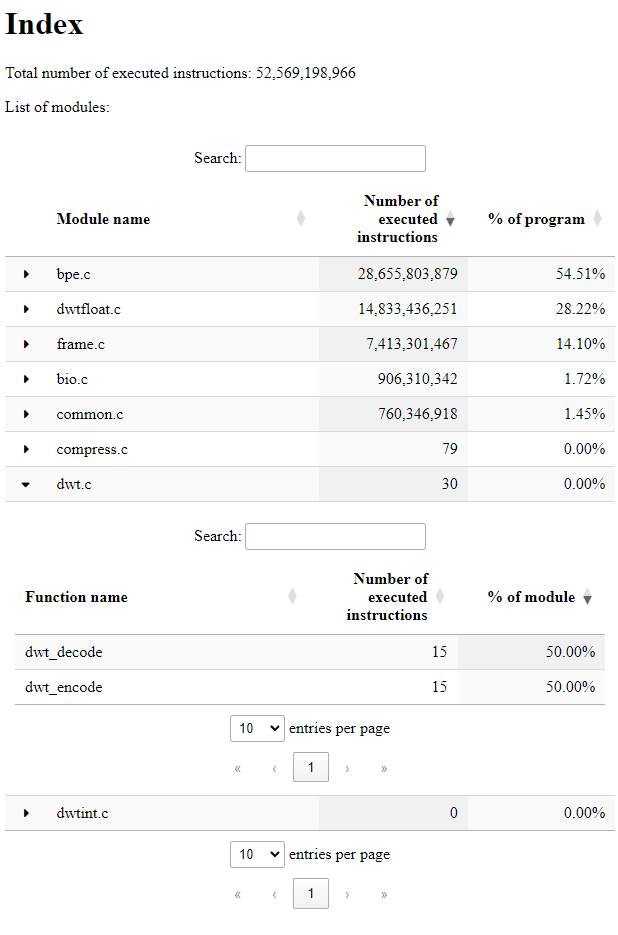
\includegraphics[width=1\textwidth]{obrazky-figures/index-table.PNG}
        \caption{A module table created from a CCSDS profile, showing each module's contribution to the total number of executed instructions. The row containing the \texttt{dwt.c} module is expanded, revealing a nested table with functions contained in this module.}
        \label{fig:index-table}
    \end{minipage}%
    \hfill%
    \begin{minipage}[t]{0.48\textwidth}
        \centering
        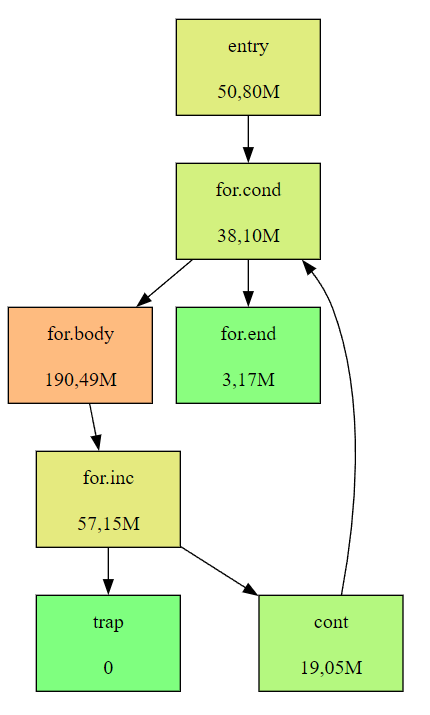
\includegraphics[width=0.8\textwidth]{obrazky-figures/cfg_update_children_types.PNG}
        \caption{A visualization \texttt{update\_parent\_types()} control flow graph. The nodes are colored based on their contribution to the total number of instructions executed in this function. The nodes also contain the approximate number of instructions executed in each block.}
        \label{fig:function-cfg}
    \end{minipage}
\end{figure}


\begin{figure}
    \centering
    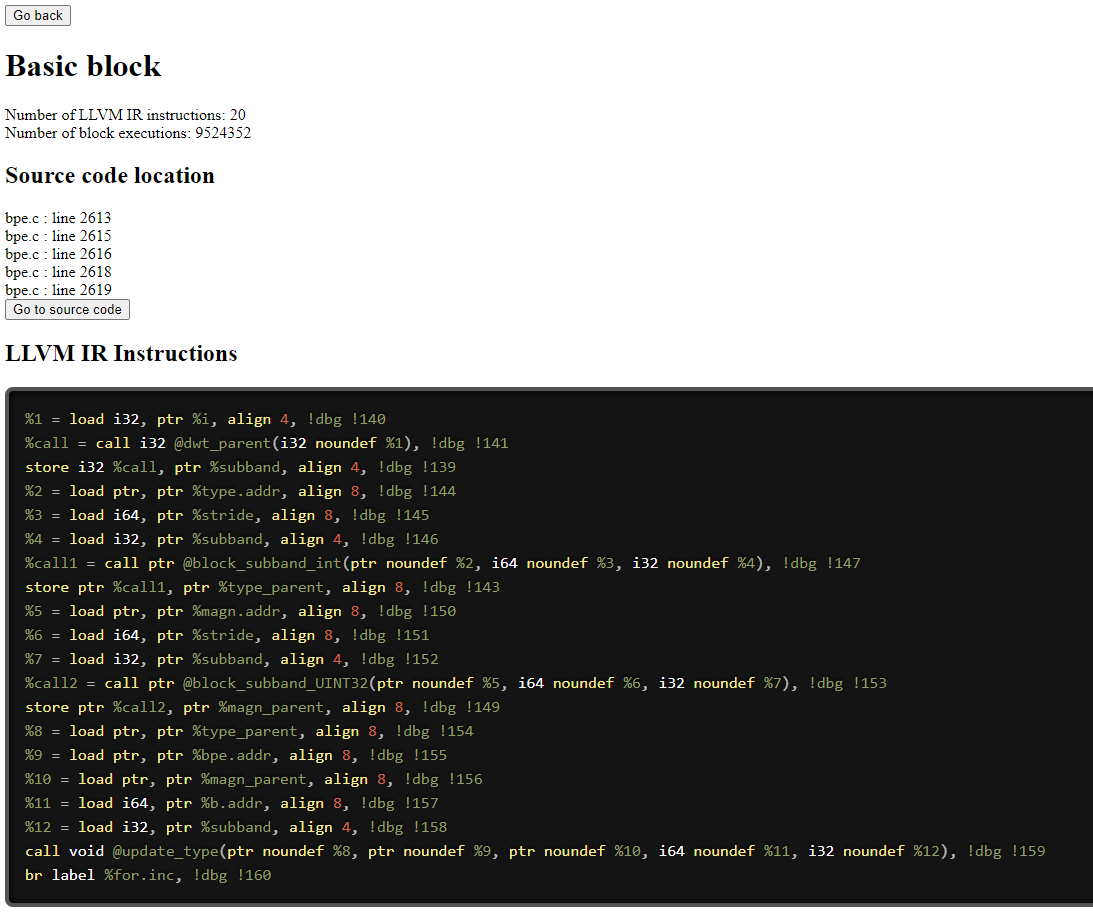
\includegraphics[scale=0.5]{obrazky-figures/update_parent_types_detail.png}
    \caption{Detail of the \texttt{for.body} basic block in the \texttt{update\_parent\_types()} function.}
    \label{fig:block-detail}
\end{figure}


\begin{figure}
    \centering
    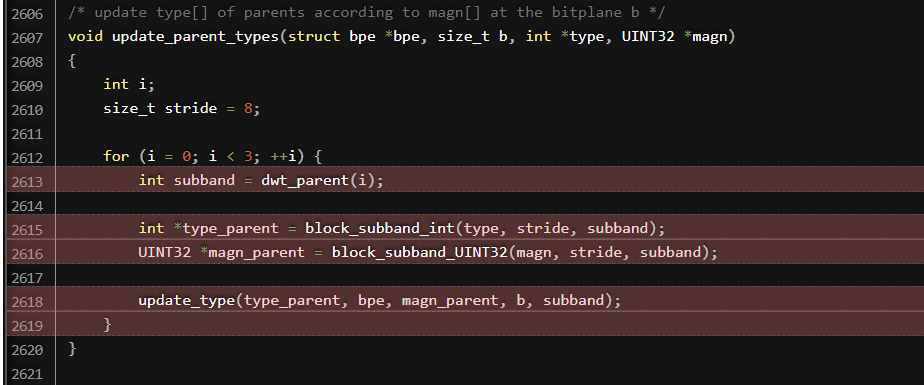
\includegraphics[scale=0.6]{obrazky-figures/update_parent_types_code.png}
    \caption{Source code of the \texttt{update\_parent\_types()} function, with the lines of the \texttt{for.body} basic block highlighted.}
    \label{fig:code-highlight}
\end{figure}


\chapter{Comparison with Established Tools}
\label{compare}
The performance of the implemented profiler was comparatively evaluated against two established open-source tools, which also contain an option to collect basic block execution counts. Although these tools also gather other information, making true apples-to-apples comparison challenging, this analysis still serves as a valuable benchmark. It shows how the new profiler would perform in real-world scenarios when used by a user specifically interested in profiling basic block execution counts.



\section{Callgrind}
Callgrind is a profiling tool based on dynamic binary instrumentation. It is a part of the Valgrind tool suite. By default, it collects the number of instructions executed, their relationship to source code lines, caller/callee relationships between functions, and the number of calls. Like all Valgrind tools, Callgrind does not run the profiled program directly on the CPU. Instead, it runs the program on a simulated CPU. It uses a disassemble-and-resynthesize approach, converting machine code to its internal intermediate representation, performing instrumentation and optimizations, and recompiling back to machine code. Since it is primarily designed to be a heavyweight profiling tool, the overhead compared to our solution is very high, as shown by Table \ref{tab:ccsds-callgrind}, being similar to the very first, slowest version described in Section \ref{hashtable-impl}. Since it is a dynamic binary instrumentation tool, Callgrind does not require recompilation or any special setup, making it very convenient to use. However, in scenarios when a user wants to perform many profiling runs on different inputs, and the program has a long runtime, this convenience might not be relevant when compared to the enormous amount of time taken by the profiling. \cite{valgrind}

\begin{table}[t]
    \centering
    \begin{tabular}{lrrrrr}
    \multicolumn{1}{l}{\multirow{2}{*}{\textbf{Image}}} & \multicolumn{1}{c}{\multirow{2}{*}{\textbf{Orig. time [s]}}} & \multicolumn{2}{c}{\textbf{Callgrind}} & \multicolumn{2}{c}{\textbf{Implemented profiler}} \\
    \cline{3-6} 
    \multicolumn{1}{l}{} & \multicolumn{1}{c}{} & \multicolumn{1}{c}{\textbf{Time [s]}} & \multicolumn{1}{c}{\textbf{Overhead}} & \multicolumn{1}{c}{\textbf{Time [s]}} & \multicolumn{1}{c}{\textbf{Overhead}} \\ 
    \hline
    \hline
    cdf97-psi.pgm & 0.029 & 1.580 & 54.48x & 0.032 & 1.10x \\
    Babboon.pgm & 0.028 & 1.574 & 56.21x  & 0.033 & 1.18x \\
    P1010042.pgm & 0.038 & 1.984 & 52.21x & 0.041 & 1.08x \\
    frame.pgm & 0.254 & 12.155 & 47.85x & 0.303 & 1.19x \\
    g10.pgm & 0.768 & 37.947 & 49.41x & 0.871 & 1.13x \\
    m612-be.pgm & 1.339 & 63.120 & 47.14x & 1.586 & 1.18x \\
    \hline
    \multicolumn{1}{l}{Average} & & & \textbf{51.22x} & & \textbf{1.14x} \\
    \end{tabular}
    \caption{A comparison of profiling overhead of Callgrind versus the optimized version of the implemented profiler, measured on the CCSDS project.}
    \label{tab:ccsds-callgrind}
\end{table}


\section{gprof}


\texttt{gprof} is a lightweight, compile-time-instrumentation-based profiler, activated by using the \texttt{-pg} option in the \texttt{gcc} or \texttt{clang} compilers. Internally, its basic block execution counting mechanism works very similarly to our solution, placing static counter arrays into every object file. However, it also uses sampling to collect information about time spent in functions and constructs a dynamic call graph based on the actual execution paths. \cite{gprof-man, gprof-paper}

Table \ref{tab:ccsds-gprof} shows the overhead comparison between the implemented profiler and \texttt{gprof} on the CCSDS project. Table \ref{tab:cpython-gprof} contains the same comparison on CPython.
 

\begin{table}[]
    \centering
    \begin{tabular}{lrrrrr}
     \multicolumn{1}{l}{\multirow{2}{*}{\textbf{Image}}} & \multicolumn{1}{c}{\multirow{2}{*}{\textbf{Orig. time [s]}}} & \multicolumn{2}{c}{\textbf{gprof}} & \multicolumn{2}{c}{\textbf{Implemented profiler}} \\
    \cline{3-6} 
    \multicolumn{1}{l}{} & \multicolumn{1}{c}{} & \multicolumn{1}{c}{\textbf{Time [s]}} & \multicolumn{1}{c}{\textbf{Overhead}} & \multicolumn{1}{c}{\textbf{Time [s]}} & \multicolumn{1}{c}{\textbf{Overhead}} \\ 
    \hline
    \hline
    cdf97-psi.pgm & 0.029 & 0.065 & 2.24x & 0.032 & 1.10x \\
    Babboon.pgm & 0.028 & 0.066 & 2.36x  & 0.033 & 1.18x \\
    P1010042.pgm & 0.038 & 0.086 & 2.26x & 0.041 & 1.08x \\
    frame.pgm & 0.254 & 0.596 & 2.35x & 0.303 & 1.19x \\
    g10.pgm & 0.768 & 1.627 & 2.12x & 0.871 & 1.13x \\
    m612-be.pgm & 1.339 & 3.120 & 2.33x & 1.586 & 1.18x \\
    \hline
    \multicolumn{1}{l}{Average} & & & \textbf{2.28x} & & \textbf{1.14x} \\
    \end{tabular}
    \caption{A comparison of profiling overhead of \texttt{gprof} versus the optimized version of the implemented profiler on the CCSDS project (optimization level \texttt{-O3}).}
    \label{tab:ccsds-gprof}
\end{table}


\begin{table}[H]
    \centering
    \begin{tabular}{lrrrrr}
    \multicolumn{1}{l}{\multirow{2}{*}{\textbf{Benchmark}}} & \multicolumn{1}{c}{\multirow{2}{*}{\textbf{Orig. time [s]}}} & \multicolumn{2}{c}{\textbf{gprof}} & \multicolumn{2}{c}{\textbf{Implemented profiler}} \\
    \cline{3-6} 
    \multicolumn{1}{l}{} & \multicolumn{1}{c}{} & \multicolumn{1}{c}{\textbf{Time [s]}} & \multicolumn{1}{c}{\textbf{Overhead}} & \multicolumn{1}{c}{\textbf{Time [s]}} & \multicolumn{1}{c}{\textbf{Overhead}} \\ 
    \hline
    \hline
    Math & 56.76 & 79.73 & 1.40x & 74.97 & 1.32x \\
    Regex & 95.59 & 124.82 & 1.31x  & 110.18 & 1.15x \\
    Scimark & 122.58 & 215.49 & 1.76x & 149.66 & 1.22x \\
    Apps & 510.51 & 803.48 & 1.57x & 604.03 & 1.18x \\
    Serialize & 594.07 & 914.59 & 1.54x & 699.96 & 1.18x \\
    \hline
    \multicolumn{1}{l}{Average} & & & \textbf{1.52x} & & \textbf{1.21x} \\
    \end{tabular}
    \caption{A comparison of profiling overhead of \texttt{gprof} versus the optimized version of the implemented profiler on the CPython interpreter (optimization level \texttt{-O3}).}
    \label{tab:cpython-gprof}
\end{table}



\chapter{Conclusion}
\label{conclusion}

This work aimed to extend the Perun tool suite by implementing a new collector based on compile-time instrumentation. This collector is a lightweight, low-overhead alternative to the \emph{Trace} collector, focusing on profiling basic block execution counts. The implementation uses the LLVM Pass Framework to perform the instrumentation. The profiler was designed to easily integrate into build systems like CMake or Unix Makefiles by setting environment variables and using a custom linker. The runtime overhead was reduced using several optimization methods, including inlining instrumentation code and control flow graph analysis to limit the number of instrumentation points without sacrificing the accuracy of the resulting profile. An interactive visualization was implemented to interpret the profiles. The performance of the profiler was evaluated on two C projects, the CCSDS image compressing algorithm, and the CPython interpreter. The results show that the overhead was reduced by about 98\% compared to the initial version. The optimized version of the profiler has achieved an overhead of about 14\% on CPython, proving that the profiler scales well and is usable even for larger projects. The profiler was evaluated against two existing open-source profilers, achieving lower overhead than even the \texttt{gprof} profiler, which utilizes similar profiling principles.

\medskip
\noindent
\textbf{Future work.} The CFG-based optimizations could be extended with path profiling, such as the Ball-Larus efficient profiling algorithm \cite{ball-larus}. Next, the existing pattern-finding algorithms could be made more efficient to reduce the impact on compile time. Furthermore, the implemented visualization could be extended to use column number information to visualize the information more accurately when there are more basic blocks on a single line. The format of the output files could be adjusted to reduce their size. Lastly, the profiler will be integrated into the Perun tool suite as a new collector.

%=========================================================================

% For compilation piecewise (see projekt.tex), it is necessary to uncomment it
% \end{document}
  \else
    \input{projekt-01-kapitoly-chapters}
  \fi
  
  % Kompilace po částech (viz výše, nutno odkomentovat a zakomentovat input výše)
  % Compilation piecewise (see above, it is necessary to uncomment it and comment out input above)
  %\subfile{chapters/projekt-01-uvod-introduction}
  % ...
  %\subfile{chapters/projekt-05-zaver-conclusion}

  % Pouzita literatura / Bibliography
  % ----------------------------------------------
\ifslovak
  \makeatletter
  \def\@openbib@code{\addcontentsline{toc}{chapter}{Literatúra}}
  \makeatother
  \bibliographystyle{bib-styles/Pysny/skplain}
\else
  \ifczech
    \makeatletter
    \def\@openbib@code{\addcontentsline{toc}{chapter}{Literatura}}
    \makeatother
    \bibliographystyle{bib-styles/Pysny/czplain}
  \else 
    \makeatletter
    \def\@openbib@code{\addcontentsline{toc}{chapter}{Bibliography}}
    \makeatother
    \bibliographystyle{bib-styles/Pysny/enplain}
  %  \bibliographystyle{alpha}
  \fi
\fi
  \begin{flushleft}
  \bibliography{projekt-20-literatura-bibliography}
  \end{flushleft}

  % vynechani stranky v oboustrannem rezimu
  % Skip the page in the two-sided mode
  \iftwoside
    \cleardoublepage
  \fi

  % Prilohy / Appendices
  % ---------------------------------------------
  \appendix
\ifczech
  \renewcommand{\appendixpagename}{Přílohy}
  \renewcommand{\appendixtocname}{Přílohy}
  \renewcommand{\appendixname}{Příloha}
\fi
\ifslovak
  \renewcommand{\appendixpagename}{Prílohy}
  \renewcommand{\appendixtocname}{Prílohy}
  \renewcommand{\appendixname}{Príloha}
\fi
%  \appendixpage

% vynechani stranky v oboustrannem rezimu
% Skip the page in the two-sided mode
%\iftwoside
%  \cleardoublepage
%\fi
  
\ifslovak
%  \section*{Zoznam príloh}
%  \addcontentsline{toc}{section}{Zoznam príloh}
\else
  \ifczech
%    \section*{Seznam příloh}
%    \addcontentsline{toc}{section}{Seznam příloh}
  \else
%    \section*{List of Appendices}
%    \addcontentsline{toc}{section}{List of Appendices}
  \fi
\fi
  \startcontents[chapters]
  \setlength{\parskip}{0pt} 
  % seznam příloh / list of appendices
  % \printcontents[chapters]{l}{0}{\setcounter{tocdepth}{2}}
  
  \ifODSAZ
    \setlength{\parskip}{0.5\bigskipamount}
  \else
    \setlength{\parskip}{0pt}
  \fi
  
  % vynechani stranky v oboustrannem rezimu
  \iftwoside
    \cleardoublepage
  \fi
  
  % Přílohy / Appendices
  \ifenglish
    \input{projekt-30-prilohy-appendices-en}
  \else
    \input{projekt-30-prilohy-appendices}
  \fi
  
  % Kompilace po částech (viz výše, nutno odkomentovat)
  % Compilation piecewise (see above, it is necessary to uncomment it)
  %\subfile{projekt-30-prilohy-appendices}
  
\end{document}
